% Options for packages loaded elsewhere
\PassOptionsToPackage{unicode}{hyperref}
\PassOptionsToPackage{hyphens}{url}
\PassOptionsToPackage{dvipsnames,svgnames,x11names}{xcolor}
\documentclass[
  11pt,
]{article}
\usepackage{xcolor}
\usepackage[margin=1in]{geometry}
\usepackage{amsmath,amssymb}
\setcounter{secnumdepth}{-\maxdimen} % remove section numbering
\usepackage{iftex}
\ifPDFTeX
  \usepackage[T1]{fontenc}
  \usepackage[utf8]{inputenc}
  \usepackage{textcomp} % provide euro and other symbols
\else % if luatex or xetex
  \usepackage{unicode-math} % this also loads fontspec
  \defaultfontfeatures{Scale=MatchLowercase}
  \defaultfontfeatures[\rmfamily]{Ligatures=TeX,Scale=1}
\fi
\usepackage{lmodern}
\ifPDFTeX\else
  % xetex/luatex font selection
\fi
% Use upquote if available, for straight quotes in verbatim environments
\IfFileExists{upquote.sty}{\usepackage{upquote}}{}
\IfFileExists{microtype.sty}{% use microtype if available
  \usepackage[]{microtype}
  \UseMicrotypeSet[protrusion]{basicmath} % disable protrusion for tt fonts
}{}
\makeatletter
\@ifundefined{KOMAClassName}{% if non-KOMA class
  \IfFileExists{parskip.sty}{%
    \usepackage{parskip}
  }{% else
    \setlength{\parindent}{0pt}
    \setlength{\parskip}{6pt plus 2pt minus 1pt}}
}{% if KOMA class
  \KOMAoptions{parskip=half}}
\makeatother
\usepackage{longtable,booktabs,array}
\usepackage{calc} % for calculating minipage widths
% Correct order of tables after \paragraph or \subparagraph
\usepackage{etoolbox}
\makeatletter
\patchcmd\longtable{\par}{\if@noskipsec\mbox{}\fi\par}{}{}
\makeatother
% Allow footnotes in longtable head/foot
\IfFileExists{footnotehyper.sty}{\usepackage{footnotehyper}}{\usepackage{footnote}}
\makesavenoteenv{longtable}
\usepackage{graphicx}
\usepackage{float}
\makeatletter
\newsavebox\pandoc@box
\newcommand*\pandocbounded[1]{% scales image to fit in text height/width
  \sbox\pandoc@box{#1}%
  \Gscale@div\@tempa{\textheight}{\dimexpr\ht\pandoc@box+\dp\pandoc@box\relax}%
  \Gscale@div\@tempb{\linewidth}{\wd\pandoc@box}%
  \ifdim\@tempb\p@<\@tempa\p@\let\@tempa\@tempb\fi% select the smaller of both
  \ifdim\@tempa\p@<\p@\scalebox{\@tempa}{\usebox\pandoc@box}%
  \else\usebox{\pandoc@box}%
  \fi%
}
% Set default figure placement to htbp
\def\fps@figure{htbp}
\makeatother
\setlength{\emergencystretch}{3em} % prevent overfull lines
\providecommand{\tightlist}{%
  \setlength{\itemsep}{0pt}\setlength{\parskip}{0pt}}
\graphicspath{{figures/}{../figures/outputs/}}
\usepackage{bookmark}
\IfFileExists{xurl.sty}{\usepackage{xurl}}{} % add URL line breaks if available
\urlstyle{same}
\hypersetup{
  pdftitle={Benchmarking TCR--pMHC structure prediction without multiple sequence alignments: a protein language model matches AlphaFold 3{,} and their disagreement predicts accuracy},
  pdfauthor={[Author list to be completed]},
  pdfkeywords={T cell receptor, peptide-MHC, structure
prediction, AlphaFold 3, protein language model, DockQ, benchmark},
  colorlinks=true,
  linkcolor={blue},
  filecolor={Maroon},
  citecolor={Blue},
  urlcolor={Blue},
  pdfcreator={LaTeX via pandoc}}

\title{Benchmarking TCR--pMHC structure prediction without multiple
sequence alignments: a protein language model matches AlphaFold 3, and
their disagreement predicts accuracy}
\author{[Author list to be completed]}
\date{28 August 2026}

\begin{document} \maketitle \begin{abstract} T cell receptor (TCR)
recognition of peptide--MHC (pMHC) is the central specificity event of
cellular immunity, and structure prediction is now the main route to
modelling it at scale. Published benchmarks agree that
multiple-sequence-alignment (MSA)-based predictors, and AlphaFold 3 in
particular, lead the field, and that protein-language-model (PLM)
predictors trail them. We revisited that conclusion on a benchmark of
136 TCR--pMHC entries released after the 30 September 2021 training
cutoff shared by every method tested, of which 126 (111 class I, 15
class II) carry a scoreable experimental reference. All methods
received byte-identical truncated inputs and a single fixed chain
convention, and every model was scored with an explicit identity chain
mapping against the same experimental references, cropped from the
deposited coordinates to the input sequence and verified to draw all
chains from a single author-defined assembly. AlphaFold 3 (median
Global DockQ 0.751) and ESMFold2, a single-sequence diffusion
predictor conditioned on a 6-billion-parameter language model rather
than on an MSA (0.736), were statistically indistinguishable (paired
Wilcoxon p = 0.68); both exceeded Protenix (0.701, p = 0.045 and p =
0.0009) and the TCR-specialised TCRmodel2 (0.708 on the 111 class I
targets) was not separable from either. Equal accuracy did not mean
equivalent behaviour. ESMFold2's ipTM tracked accuracy far more
tightly than AlphaFold 3's (Pearson r = 0.79 vs 0.66); AlphaFold 3 was
more sensitive to reference resolution; and the two models placed the
TCR more than 90\ensuremath{^{\circ}} apart on 10 of 126 complexes
while agreeing on the pMHC to within 0.44 \AA{}. The
C\ensuremath{\alpha} RMSD between the two predictions --- a quantity
computable without any experimental structure --- predicted the worse
of the two DockQ scores better than either model's own confidence
(Spearman \ensuremath{\rho} = \ensuremath{-}0.884 vs +0.60 and +0.64),
and the two methods together reached medium-or-better accuracy on 119
of 126 complexes against 107 and 115 individually. Instrumenting both
samplers showed the equal accuracy is reached by different routes:
AlphaFold 3 is still 44 \AA{} from its answer at the midpoint of
denoising and converges only in the final fifth of its schedule,
whereas ESMFold2 is within 6 \AA{} at its midpoint. Exploiting that,
cutting AlphaFold 3 from 200 to 160 denoising steps and from 5
diffusion samples to 1 gave a 1.80\ensuremath{\times} speed-up on 30
complexes at a cost of \ensuremath{-}0.010 Global DockQ (95\% CI
\ensuremath{-}0.032 to +0.007, p = 0.33). We conclude that MSAs are
not required for state-of-the-art TCR--pMHC modelling, that
cross-architecture agreement is a strong reference-free quality
signal, and that the default AlphaFold 3 sampler is substantially
over-provisioned for complexes of this size. \end{abstract}

\section{1 Introduction}\label{introduction}

The \ensuremath{\alpha}\ensuremath{\beta} T cell receptor recognises a short peptide presented by a major
histocompatibility complex (MHC) protein, and the geometry of that
engagement --- the docking angle of the TCR variable domains over the
peptide-binding platform, and the conformations of the six
complementarity-determining region (CDR) loops that contact the peptide
--- determines specificity. Experimental determination of TCR--pMHC
complexes remains slow relative to the size of the repertoire, so
computational modelling has become the practical route to structural
hypotheses at scale, whether for epitope-specificity prediction, TCR
engineering, or immunotherapeutic design [1--3].

Deep-learning structure prediction transformed this problem twice.
AlphaFold 2 made accurate single-chain and many multi-chain predictions
routine [4], though early benchmarks identified adaptive immune
recognition --- antibody--antigen and TCR--pMHC complexes in particular
--- as a systematic failure mode [5]. AlphaFold 3 replaced the
Structure Module with a diffusion head and reported substantially
improved interface accuracy across biomolecular space [6], and
TCR-specific adaptations such as TCRdock [7] and TCRmodel2 [8]
narrowed the gap for this class of complex specifically. In parallel,
protein language models made structure prediction possible without an
MSA at all: ESMFold demonstrated that a sufficiently large language
model encodes atomic-level structure in its representations [9],
trading evolutionary coupling signal for a learned prior and an
order-of-magnitude speed-up.

Recent TCR--pMHC benchmarks have converged on a consistent ranking. Lu
et al. evaluated thirteen methods on 70 post-cutoff complexes and
concluded that ``MSA-based methods, particularly AlphaFold3,
consistently outperform all alternatives'', with most PLM-based models
underperforming except a PLM variant built on an AlphaFold-3-style
architecture [10]. Ascunce-París et al.~reached the same conclusion
on 265 class I complexes, reporting AlphaFold 3 as the best generaliser
to post-training structures [11]. Shi et al.~found that TCR-specific
tools derived from AlphaFold 2 gain interface accuracy at the cost of
framework accuracy, and that CDR3 loops, docking orientation and class
II MHC--peptide interfaces remain difficult for every method [12].
Yin et al.~observed complementary behaviour between methods and pooling
gains for antibody--peptide complexes [13]. Together these establish
the field's working assumption: evolutionary information is what makes
TCR--pMHC prediction work.

Two considerations motivate re-examining that conclusion. First, the PLM
predictors in those comparisons are predominantly ESMFold-generation
models whose structure module is a direct AlphaFold-2 descendant,
whereas a current-generation language-model predictor with a diffusion
structure head is a substantially different architecture. Second, a
benchmark that ranks methods addresses only part of the question. Where
two architectures that share little on the conditioning side --- one
using a paired MSA and structural templates, the other only the query
sequence --- achieve comparable accuracy, the more informative questions
concern the route each takes to that accuracy and whether the
disagreements between them carry usable information.

Here we assemble a benchmark of 136 TCR--pMHC entries released after
30 September 2021, the training cutoff shared by AlphaFold 3, Protenix
and ESMFold2, of which 126 carry a scoreable experimental reference.
Every method receives identical truncated inputs under one chain
convention, and every prediction is scored against a native cropped
from the deposited coordinates and audited to come from a single
author-defined assembly. We report interface accuracy (DockQ),
TCR-specific accuracy (MHC-aligned weighted all-CDR
C\ensuremath{\alpha} RMSD and framework-aligned CDR3 all-atom RMSD),
confidence calibration, sensitivity to reference resolution and to
training-set similarity, the structural anatomy of the disagreement
between the two leading models, the internal trajectories of both
diffusion samplers, and the wall-clock cost of the default AlphaFold 3
sampler settings.

\section{2 Materials and methods}\label{materials-and-methods}

\subsection{2.1 Benchmark set
construction}\label{benchmark-set-construction}

We constructed a dataset of TCR-pMHC Class I and Class II complexes from the TCR3d database [1,3], which
curates all known TCR complex structures. Restricting to \ensuremath{\alpha}\ensuremath{\beta} TCR complexes
with an initial RCSB release date after 30 September 2021 gave 427 class
I and 72 class II candidates. Of these, 136 were complete
TCR--peptide--MHC complexes containing all of an MHC peptide-binding
platform, a peptide, and paired TCR \ensuremath{\alpha} and \ensuremath{\beta} variable domains (114 class
I, 22 class II); the remainder were unliganded TCRs, pMHC-only entries,
TCR-mimic antibody complexes, or otherwise incomplete triads.

All 136 entries were reviewed against their deposited coordinates and
primary publications, and ten were excluded from scoring. Five (8TRL,
8TRQ, 8TRR, 9NIG, 9WNT) contain modified peptide residues that a
standard FASTA sequence cannot represent, and because the modification
is in every case part of the interaction being modelled, predicting
these complexes from sequence alone is not well posed. Four (8VD0,
8VQ8, 9AUD, 9C3E) are engineered constructs in which the peptide is
covalently fused to the MHC through a linker; modelling their
components as separate chains would alter the connectivity of the
experiment. The last, 9J4S, has no physical TCR--pMHC interface in any
author-defined assembly of the deposited structure and so cannot be
scored at all. This leaves 126 scoreable complexes, 111 class I and 15
class II.

No redundancy filter or resolution cut was applied to the primary set.
TCR variable-domain identity is a poor novelty axis --- germline V-gene
framework dominates a \textasciitilde110-residue V domain --- and
filtering on it discards most of the set while retaining an
idiosyncratic remainder (Section 3.10). Instead, similarity to the
pre-cutoff structural record is measured explicitly and treated as a
covariate.

\subsection{2.2 Domain truncation and chain
convention}\label{domain-truncation-and-chain-convention}

Each complex was truncated to the domains that constitute the variable
regions of the TCR--pMHC interface (Figure 1). For class I, \ensuremath{\beta}2-microglobulin was removed and the
MHC heavy chain was cut to its \ensuremath{\alpha}1\ensuremath{\alpha}2 peptide-binding platform (median 181
residues, range 161--181); for class II, the \ensuremath{\alpha}1 and \ensuremath{\beta}1 domains were
retained (81--85 and 89--93 residues). TCR chains were cut to their
variable domains (\ensuremath{\alpha} 101--114 residues, \ensuremath{\beta} 105--116). Prediction inputs
used the complete deposited polymer sequences over those spans.

Every method received the same chain letters, with no per-model
remapping anywhere in the pipeline: for class I, MHC \ensuremath{\alpha}1\ensuremath{\alpha}2 (A), peptide
(B), TCR\ensuremath{\alpha} (C) and TCR\ensuremath{\beta} (D); for class II, MHC-II\ensuremath{\alpha} (A), peptide (B),
MHC-II\ensuremath{\beta} (C), TCR\ensuremath{\alpha} (D) and TCR\ensuremath{\beta} (E).

\begin{figure}[H]
\centering
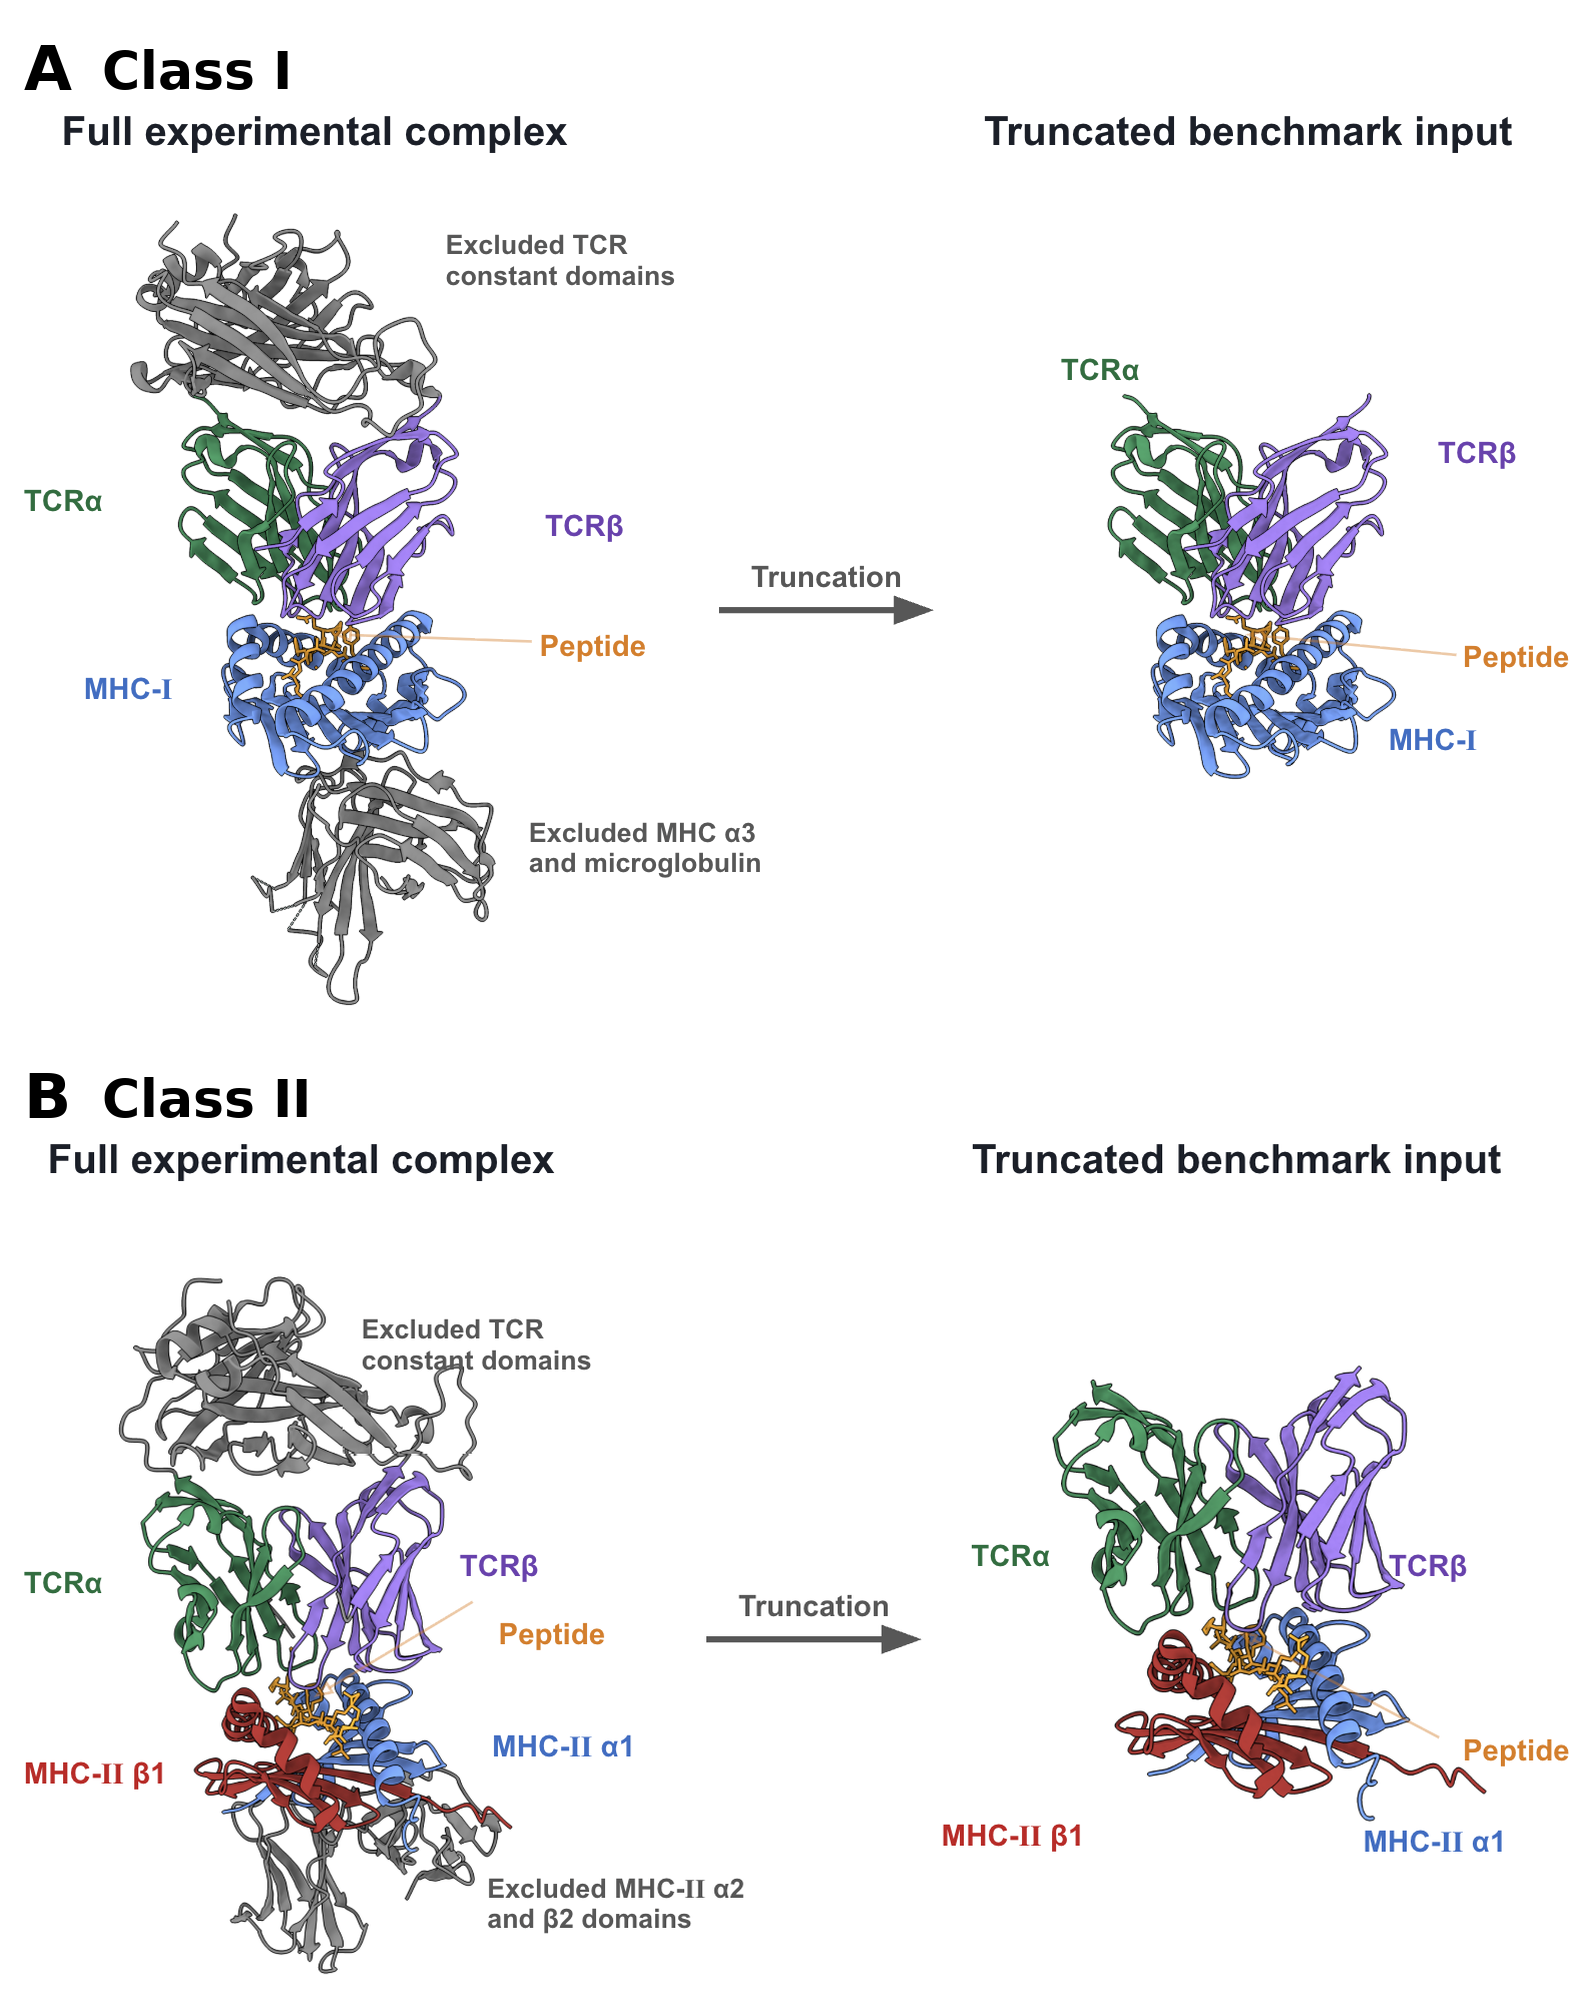
\includegraphics[width=0.85\linewidth,height=\textheight,keepaspectratio,alt={Domain truncation applied to the benchmark complexes. (A) Class I. The TCR constant domains, the MHC \ensuremath{\alpha}3 domain and \ensuremath{\beta}2-microglobulin are removed, leaving the MHC-I \ensuremath{\alpha}1\ensuremath{\alpha}2 peptide-binding platform, the peptide and the paired TCR variable domains. (B) Class II. The TCR constant domains and the MHC-II \ensuremath{\alpha}2 and \ensuremath{\beta}2 domains are removed, leaving the \ensuremath{\alpha}1 and \ensuremath{\beta}1 peptide-binding domains, the peptide and the paired TCR variable domains. Retained chains are coloured by role; removed regions are grey.}]{Figure_truncation.png}
\caption{\textbf{Domain truncation applied to the benchmark complexes.}
(\textbf{A}) Class I. The TCR constant domains, the MHC \ensuremath{\alpha}3 domain and
\ensuremath{\beta}2-microglobulin are removed, leaving the MHC-I \ensuremath{\alpha}1\ensuremath{\alpha}2 peptide-binding
platform, the peptide and the paired TCR variable domains. (\textbf{B})
Class II. The TCR constant domains and the MHC-II \ensuremath{\alpha}2 and \ensuremath{\beta}2 domains are
removed, leaving the \ensuremath{\alpha}1 and \ensuremath{\beta}1 peptide-binding domains, the peptide and
the paired TCR variable domains. Retained chains are coloured by role;
removed regions are grey.}
\end{figure}

\subsection{2.3 Structure prediction
methods}\label{structure-prediction-methods}

Four methods were run on identical inputs.

AlphaFold 3 [6] predictions were obtained through the AlphaFold
Server, which supplies MSAs and structural templates from its own
pipeline and returns five ranked diffusion samples; the top-ranked model
by ranking score was scored. The server enforces a 30 September 2021
training cutoff.

Protenix [22], an open reproduction of the AlphaFold 3 architecture,
was run through its public server with the same inputs, and the
top-ranked model scored.

ESMFold2 (the \texttt{biohub/ESMFold2} checkpoint, conditioned on the
\texttt{biohub/ESMC-6B} language model) [21] was run through the ESM SDK
API as model \texttt{esmfold2-fast-2026-05} with the SDK defaults of 10
refinement loops and 100 sampling steps. ESMFold2 is a diffusion
structure predictor in the same sense as AlphaFold 3, but it takes no
MSA and no structural template: its only input is the query sequence,
embedded by a 6-billion-parameter protein language model. This is the
architectural contrast on which the present comparison rests, and it is
a strict one, since the two methods share the diffusion generative head
and little else on the conditioning side.

TCRmodel2 [8] was installed locally from the Pierce laboratory
repository (AlphaFold 2.3 base,
\texttt{alphafold\_params\_2022-12-06}) with
\texttt{-\/-max\_template\_date=2021-09-30} applied explicitly to both
the TCR and the pMHC template searches; the default is effectively
unrestricted, so this setting is required for a valid post-cutoff
comparison. TCRmodel2 accepts a fixed peptide length for class II and
was therefore run on class I only, giving 111 predictions.

Mean end-to-end runtimes were 5.2 s per complex for the ESMFold2 API
(median, IQR 4.9--6.4 s) and 13.4 s per complex for a local AlphaFold 3
run at default sampler settings on one RTX PRO 6000 (Section 2.11).

\subsection{2.4 Interface accuracy}\label{interface-accuracy}

Interface accuracy was measured with DockQ v2.1.3 [14,15], run once
per complex. The primary reported quantity is
DockQ v2's Global DockQ, its interface-size weighted score over the
whole complex; per-pairwise-interface DockQ values are also retained,
giving 6 interfaces per class I complex and 10 per class II complex.
Standard CAPRI thresholds are used throughout (\textless{} 0.23
incorrect, 0.23--0.49 acceptable, 0.49--0.80 medium, \ensuremath{\geq} 0.80 high)
[16].

\subsection{2.5 CDR annotation}\label{cdr-annotation}

TCR\ensuremath{\alpha} and TCR\ensuremath{\beta} chains were annotated once per
biological sequence with ANARCI [17] under IMGT numbering [18],
and the annotation propagated to prediction and native coordinates
through pairwise sequence alignment rather than through PDB residue
numbering. CDR ranges were the inclusive IMGT intervals 27--38 (CDR1),
56--65 (CDR2), 81--86 (CDR2.5) and 104--118 (CDR3); ``all CDRs'' means
all four regions on both chains, eight in total.

\subsection{2.6 TCR-specific RMSD
metrics}\label{tcr-specific-rmsd-metrics}

Two TCR-specific metrics were computed on the same top-ranked
predictions the DockQ workflow scores; predictions were never selected
using a native RMSD. The first, the MHC-aligned weighted all-CDR C\ensuremath{\alpha} RMSD, follows the TCRdock
formulation [7,19]. MHC residues are matched between prediction and
native by sequence alignment; a single ordinary-least-squares Kabsch
superposition of the class I peptide-binding platform (or, jointly, of
both class II peptide-binding domains) is applied to the entire
predicted complex, and no further fit is performed. C\ensuremath{\alpha} RMSD is then
computed over the eight CDR regions with CDR3 residues weighted 3 and
all others weighted 1:

\[\mathrm{RMSD}_{w} = \sqrt{\frac{\sum_i w_i d_i^2}{\sum_i w_i}}\]

Because there is no second fit, this metric measures how accurately the
TCR is docked on the pMHC.

The second, the framework-aligned CDR3 all-atom RMSD, measures the
opposite quantity. For each chain independently, the predicted
variable-domain framework (the IMGT-numbered variable domain excluding
all four CDR regions) is superimposed on the native framework using
matched non-hydrogen atoms, and all-heavy-atom RMSD is then computed
over the corresponding CDR3 loop without further alignment, comparing
only identically named atoms in sequence-matched, identity-matched
residues. C\ensuremath{\alpha}-only versions are retained as quality-control columns.

\subsection{2.7 Superposition-free CDR accuracy
(lDDT)}\label{superposition-free-cdr-accuracy-lddt}

Both metrics above answer their question through a superposition, and
each superposition is a choice. The local distance difference test
(lDDT) [23] removes that choice: a residue is scored by the fraction of
its interatomic distances to the rest of the structure that the
prediction reproduces, averaged over four tolerances (0.5, 1, 2 and
4~\AA{}), counting only pairs closer than 15~\AA{} in the reference and
excluding pairs within one residue. It needs no alignment and no
reference frame, and it is bounded in [0, 1].

lDDT was computed on C\ensuremath{\alpha} atoms, which is AlphaFold's own
definition and requires no symmetric-side-chain correction; the all-atom
view of the CDRs is already carried by the framework-aligned CDR3 RMSD.
Residues were matched between prediction and native through the same
manifest-sequence alignment, and the CDRs defined by the same ANARCI
annotation, as the two RMSD metrics, so the residue sets behind the two
families of number are identical. Every TCR region was scored twice,
differing only in which atoms may act as contact partners: against every
chain of the complex, which makes the score sensitive to where the TCR is
docked, and against the CDR's own TCR chain alone, which removes the
docking and leaves local loop geometry. Whole-chain, peptide, MHC and
whole-complex lDDT are reported alongside for context.

\subsection{2.8 Metric validation and quality
control}\label{metric-validation-and-quality-control}

Every metric reports expected, matched and resolved residue counts, atom
counts, coverage fraction and a pass/fail status; incomplete loops are
kept separate from the complete-case analysis rather than silently
scored. Validation tests confirm that a native scored against itself,
and against a rigidly rotated and translated copy of itself, returns
approximately zero; that displacing an intact TCR relative to a fixed
MHC raises the MHC-aligned CDR RMSD while leaving framework-aligned CDR3
RMSDs near zero; that deforming a CDR3 loop raises its own
framework-aligned RMSD; and that permuting chain identifiers changes
nothing, because chain assignment is by sequence and biological role. The
lDDT implementation is checked against biotite's implementation of
Mariani et al.~to within $10^{-6}$, returns 1 for a structure
scored against itself and against a rigidly rotated and translated copy of
itself, and is unaffected by rigid motion of a group lying outside the
15~\AA{} inclusion radius.

\subsection{2.9 Confidence and reference-free quality
scores}\label{confidence-and-reference-free-quality-scores}

Each method's own interface confidence (ipTM, and pTM where available)
was taken from its output. Per-residue predicted lDDT (pLDDT) was read
from the B-factor column of the same top-ranked prediction file that was
scored, averaged over a residue's non-hydrogen atoms and then over a
region; all four methods write it on the 0--100 scale here, and anything
reported in [0, 1] is rescaled. Confidence is therefore compared with
accuracy residue-for-residue over exactly the residue sets of Section 2.7,
and the calibration error reported is the mean of pLDDT − lDDT over
complexes. pDockQ [20] was computed
per interface from the predicted structure and per-residue confidence,
and averaged per complex. A published random-forest quality-tier
classifier for TCR--pMHC models [11] was re-implemented against this
benchmark's chain convention and scored on all 126 complexes; the subset
of class I targets whose PDB identifiers do not appear in its training
set (n = 27) is reported separately throughout.

\subsection{2.10 A composite single-prediction confidence
score}\label{a-composite-single-prediction-confidence-score}

Each of the scores above summarises one aspect of a prediction. We
combined four of them into a single quantity, MOGGER, as their geometric
mean:

{\large
\[\mathrm{MOGGER}=\left(\min_{i\neq j}\mathrm{ipTM}_{ij}\;\cdot\;\mathrm{pDockQ}\;\cdot\;\frac{\mathrm{pLDDT}_{\mathrm{CDR3}\alpha}}{100}\;\cdot\;\frac{1}{1+\max_{i\neq j}\mathrm{PAE}^{\min}_{ij}}\right)^{1/4}\]
}

\noindent where $\mathrm{ipTM}_{ij}$ and $\mathrm{PAE}^{\min}_{ij}$ are
the off-diagonal entries of AlphaFold 3's chain-pair ipTM and chain-pair
minimum-PAE matrices, so the first and fourth terms are the weakest and
the least certain chain relationship in the complex; pDockQ is the
interface score of Section 2.9; and $\mathrm{pLDDT}_{\mathrm{CDR3}\alpha}$
is the mean pLDDT of the CDR3\ensuremath{\alpha} loop, the region that has to be right for
the TCR to dock correctly. Each term lies on the unit interval, so the
geometric mean penalises a single weak term more than an arithmetic mean
would --- a prediction is only as good as its worst-supported part.

Every input is read from one AlphaFold 3 \texttt{model\_0} prediction and
its own summary and full confidence files. No second sample, no second
architecture, no template and no reference structure enters the score,
which is what makes it usable prospectively. The formula was fixed on
this benchmark and is therefore reported as a benchmark result, not as a
validated external predictor.

\subsection{2.11 Sampler instrumentation and
timing}\label{sampler-instrumentation-and-timing}

Both models' official samplers were patched observationally to retain
the coordinate state after every production denoising step, changing no
arithmetic: AlphaFold 3's \texttt{diffusion\_head.sample} already
computes and discards the per-step positions inside its scan, and the
patch keeps them; ESMFold2's \texttt{DiffusionStructureHead.sample}
holds its state in a local, so its installed source was rewritten at a
unique anchor. Parity between instrumented and stock runs under the same
seed was verified per model (mean \textbar \ensuremath{\Delta}DockQ\textbar{} = 0.0008,
maximum 0.0122).

Sampler economy was measured on 30 complexes drawn with a frozen seed
from the 126 scoreable set (28 class I, 2 class II, 397--416 residues),
run serially on one idle RTX PRO 6000 with identical MSAs and templates
taken verbatim from the AlphaFold Server bundles the benchmark's own
predictions came from, and the same per-complex seed. Four tracks were
run: 200 steps \ensuremath{\times} 5 samples (default), 160 \ensuremath{\times} 5, 200 \ensuremath{\times} 1 and 160 \ensuremath{\times} 1. All
30 complexes fall in AlphaFold 3's 512-token bucket, so JIT compilation
and kernel autotuning happen once per track; both were charged to two
warm-up predictions run and discarded before timing. Instrumentation
costs \textasciitilde2\% and was run as a separate pass, so the baseline
track is stock AlphaFold 3.

\subsection{2.12 Statistics and software}\label{statistics-and-software}

Paired method comparisons use the Wilcoxon signed-rank test on the
complexes both methods predicted. Correlations are Pearson and Spearman
with bootstrap confidence intervals (10,000 resamples, fixed seed);
regressions use ordinary least squares with HC3 robust standard errors.

\section{3 Results}\label{results}

\subsection{3.1 Composition of the benchmark
set}\label{composition-of-the-benchmark-set}

The 126 scoreable complexes comprise 111 class I and 15 class II
entries, 112 human and 14 mouse, released between 13 October 2021 and 29
July 2026. One hundred and twenty were determined by X-ray
crystallography and six by cryo-EM, with resolutions from 1.54 to 4.44 \AA{}
(median 2.56 \AA{}, IQR 2.20--3.00 \AA{}). They span 27 distinct MHC alleles ---
the most frequent being HLA-A*02 (29), H2-Db (10), HLA-A*11 (10),
HLA-B*27 (9), HLA-A*24 (9) and HLA-E (7) --- and 79 distinct peptide
sequences of 8--15 residues (median 9).

\subsection{3.2 Overall interface
accuracy}\label{overall-interface-accuracy}

Every method produced at least an acceptable model of every complex:
Global DockQ never fell below 0.23 for any method on any of the 126
complexes (Figure 2A). Median Global DockQ was 0.751 for AlphaFold 3
(IQR 0.571--0.826), 0.736 for ESMFold2 (0.592--0.840), 0.708 for
TCRmodel2 on its 111 class I targets (0.590--0.808) and 0.701 for
Protenix (0.530--0.799).

The two leading methods are not distinguishable. Paired over all 126
complexes, AlphaFold 3 minus ESMFold2 gives a mean difference of \ensuremath{-}0.016
and a median difference of \ensuremath{-}0.002 (Wilcoxon p = 0.68). Both, however,
separate from Protenix: AlphaFold 3 +0.039 (p = 0.045) and ESMFold2
+0.055 (p = 0.0009). TCRmodel2 was not separable from any of the three
on its class I subset (all p \textgreater{} 0.23).

The CAPRI-class view (Figure 2B) tells the same story with a different
emphasis. No method produced an incorrect model. ESMFold2 placed the
largest fraction in the medium-or-better band (91.3\%: 54.0\% medium,
37.3\% high), followed by TCRmodel2 (88.3\%: 60.4\% medium, 27.9\%
high), AlphaFold 3 (84.9\%: 50.0\% medium, 34.9\% high) and Protenix
(79.4\%: 54.0\% medium, 25.4\% high). AlphaFold 3's
slightly higher median therefore coexists with a slightly heavier
acceptable-only tail than ESMFold2's --- the two distributions cross.

This result runs counter to the current consensus [10,11]: a
predictor that uses neither an MSA nor a structural template matches
AlphaFold 3 on post-cutoff TCR--pMHC complexes.

\begin{figure}
\centering
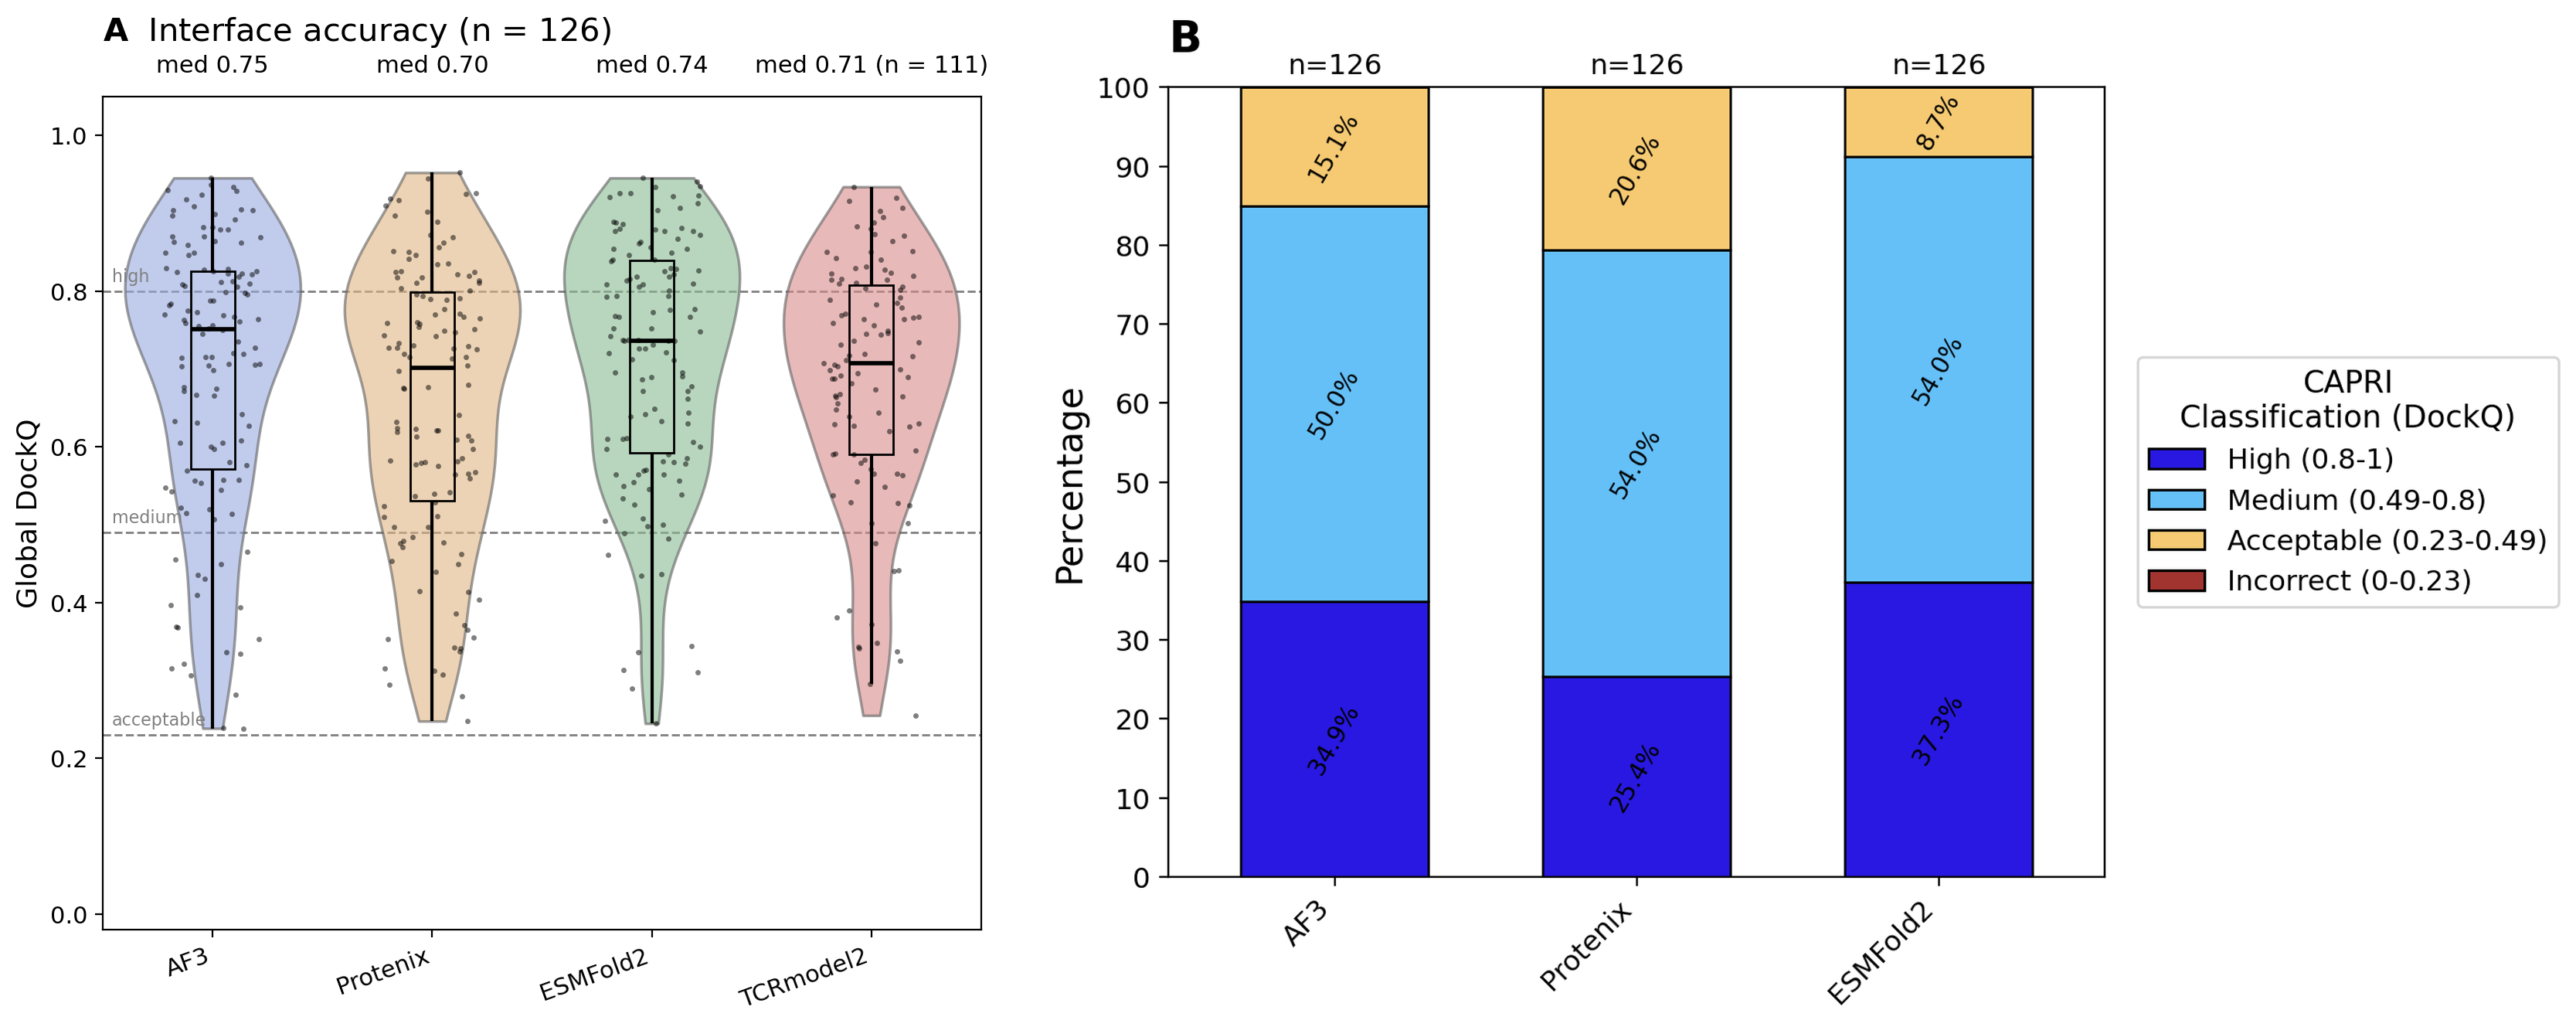
\includegraphics[width=1\linewidth,height=\textheight,keepaspectratio,alt={Interface accuracy on 126 post-cutoff TCR--pMHC complexes. (A) Distribution of Global DockQ per method; box, IQR and median; dots, individual complexes; dashed lines, CAPRI thresholds. (B) The same data as CAPRI classes, as a percentage of each method's own set. No method produced an incorrect model of any complex. TCRmodel2 covers the 111 class I complexes only, in both panels.}]{Figure_accuracy.png}
\caption{\textbf{Interface accuracy on 126 post-cutoff TCR--pMHC
complexes.} (\textbf{A}) Distribution of Global DockQ per method; box,
IQR and median; dots, individual complexes; dashed lines, CAPRI
thresholds. (\textbf{B}) The same data as CAPRI classes, as a percentage
of each method's own set. No method produced an incorrect model of any
complex. TCRmodel2 covers the 111 class I complexes only, in both
panels.}
\end{figure}

\subsection{3.3 Accuracy by interface}\label{accuracy-by-interface}

Global DockQ is weighted across all interfaces of the complex, several
of which are modelled accurately by every method. Decomposing it by
interface (Table 1) localises the differences between methods. The
MHC--peptide interface is effectively solved by every method: median
DockQ 0.940 (AlphaFold 3), 0.939 (ESMFold2), 0.933 (Protenix) and 0.931
(TCRmodel2), with the class II MHC\ensuremath{\alpha}--peptide and peptide--MHC\ensuremath{\beta}
interfaces close behind (0.90--0.91). The TCR\ensuremath{\alpha}--TCR\ensuremath{\beta} pairing is also
reliable (0.79--0.82). Everything that separates methods, and everything
that separates easy complexes from hard ones, is in the four
TCR-versus-pMHC interfaces, whose medians run 0.55--0.71. One class II
interface is a partial exception: AlphaFold 3 models the
MHC-II\ensuremath{\alpha}--MHC-II\ensuremath{\beta} heterodimer pairing itself at median DockQ 0.628,
against 0.845 for ESMFold2 and 0.789 for Protenix, the single largest
per-interface deficit for AlphaFold 3 in the table.

\begin{longtable}[]{@{}
  >{\raggedright\arraybackslash}p{(\linewidth - 10\tabcolsep) * \real{0.4444}}
  >{\raggedleft\arraybackslash}p{(\linewidth - 10\tabcolsep) * \real{0.0741}}
  >{\raggedleft\arraybackslash}p{(\linewidth - 10\tabcolsep) * \real{0.0988}}
  >{\raggedleft\arraybackslash}p{(\linewidth - 10\tabcolsep) * \real{0.1235}}
  >{\raggedleft\arraybackslash}p{(\linewidth - 10\tabcolsep) * \real{0.1235}}
  >{\raggedleft\arraybackslash}p{(\linewidth - 10\tabcolsep) * \real{0.1358}}@{}}
\caption{\textbf{Median per-interface DockQ by method.} \emph{n} is the
number of complexes contributing that interface (an interface with no
native contacts is not scored, so peptide--TCR interfaces are absent in
a few complexes whose TCR does not touch the peptide). The final row
collapses the four TCR-versus-pMHC interfaces to one value per complex,
then takes the median over complexes.}\tabularnewline
\toprule\noalign{}
\begin{minipage}[b]{\linewidth}\raggedright
Interface
\end{minipage} & \begin{minipage}[b]{\linewidth}\raggedleft
\emph{n}
\end{minipage} & \begin{minipage}[b]{\linewidth}\raggedleft
AF3
\end{minipage} & \begin{minipage}[b]{\linewidth}\raggedleft
Protenix
\end{minipage} & \begin{minipage}[b]{\linewidth}\raggedleft
ESMFold2
\end{minipage} & \begin{minipage}[b]{\linewidth}\raggedleft
TCRmodel2
\end{minipage} \\
\midrule\noalign{}
\endfirsthead
\toprule\noalign{}
\begin{minipage}[b]{\linewidth}\raggedright
Interface
\end{minipage} & \begin{minipage}[b]{\linewidth}\raggedleft
\emph{n}
\end{minipage} & \begin{minipage}[b]{\linewidth}\raggedleft
AF3
\end{minipage} & \begin{minipage}[b]{\linewidth}\raggedleft
Protenix
\end{minipage} & \begin{minipage}[b]{\linewidth}\raggedleft
ESMFold2
\end{minipage} & \begin{minipage}[b]{\linewidth}\raggedleft
TCRmodel2
\end{minipage} \\
\midrule\noalign{}
\endhead
\bottomrule\noalign{}
\endlastfoot
MHC-I -- peptide & 111 & 0.940 & 0.933 & 0.939 & 0.931 \\
MHC-II\ensuremath{\alpha} -- peptide & 15 & 0.904 & 0.911 & 0.905 & --- \\
peptide -- MHC-II\ensuremath{\beta} & 15 & 0.909 & 0.887 & 0.902 & --- \\
TCR\ensuremath{\alpha} -- TCR\ensuremath{\beta} & 126 & 0.798 & 0.800 & 0.821 & 0.791 \\
MHC-II\ensuremath{\alpha} -- MHC-II\ensuremath{\beta} & 15 & 0.628 & 0.789 & 0.845 & --- \\
MHC-I -- TCR\ensuremath{\alpha} & 111 & 0.672 & 0.590 & 0.653 & 0.644 \\
MHC-I -- TCR\ensuremath{\beta} & 110 & 0.686 & 0.551 & 0.696 & 0.611 \\
peptide -- TCR\ensuremath{\alpha} & 120 & 0.710 & 0.605 & 0.676 & 0.641 \\
peptide -- TCR\ensuremath{\beta} & 122 & 0.687 & 0.633 & 0.690 & 0.681 \\
MHC-II\ensuremath{\alpha} -- TCR\ensuremath{\alpha} & 11 & 0.615 & 0.600 & 0.714 & --- \\
MHC-II\ensuremath{\alpha} -- TCR\ensuremath{\beta} & 12 & 0.773 & 0.767 & 0.839 & --- \\
MHC-II\ensuremath{\beta} -- TCR\ensuremath{\alpha} & 15 & 0.720 & 0.687 & 0.819 & --- \\
MHC-II\ensuremath{\beta} -- TCR\ensuremath{\beta} & 15 & 0.719 & 0.519 & 0.764 & --- \\
\textbf{All TCR--pMHC interfaces (per complex)} & 126 & \textbf{0.692} &
\textbf{0.621} & \textbf{0.694} & \textbf{0.632} \\
\end{longtable}

Collapsing those four interfaces to one value per complex, median
TCR-versus-pMHC DockQ is 0.694 for ESMFold2, 0.692 for AlphaFold 3,
0.632 for TCRmodel2 and 0.621 for Protenix. On this stricter reading the
acceptable-or-better rate falls from 100\% to 92.9\% (ESMFold2), 90.1\%
(TCRmodel2), 87.3\% (AlphaFold 3) and 84.1\% (Protenix), and the
high-accuracy rate is 28.6\%, 27.8\%, 19.8\% and 17.5\% respectively.
Approximately one complex in ten is therefore still docked incorrectly
by the best-performing methods.

\subsection{3.4 TCR-specific accuracy: docking versus CDR3 loop
conformation}\label{tcr-specific-accuracy-docking-versus-cdr3-loop-conformation}

The two TCR-specific metrics decompose that residual error (Table 2).

\begin{longtable}[]{@{}
  >{\raggedright\arraybackslash}p{(\linewidth - 8\tabcolsep) * \real{0.3793}}
  >{\raggedright\arraybackslash}p{(\linewidth - 8\tabcolsep) * \real{0.1552}}
  >{\raggedright\arraybackslash}p{(\linewidth - 8\tabcolsep) * \real{0.1552}}
  >{\raggedright\arraybackslash}p{(\linewidth - 8\tabcolsep) * \real{0.1552}}
  >{\raggedright\arraybackslash}p{(\linewidth - 8\tabcolsep) * \real{0.1552}}@{}}
\caption{\textbf{TCR-specific structural accuracy, median (IQR) in
\aa{}ngströms, class I and II pooled.} The MHC-aligned metric applies one
rigid superposition of the predicted MHC peptide-binding platform onto
the native and then measures all eight CDRs with CDR3 residues weighted
3, so it reports docking accuracy. The framework-aligned metrics fit
each TCR chain's variable-domain framework independently and then
measure the CDR3 loop, so they report loop accuracy independent of
docking. TCRmodel2 is scored on its 111 class I
predictions.}\tabularnewline
\toprule\noalign{}
\begin{minipage}[b]{\linewidth}\raggedright
Metric
\end{minipage} & \begin{minipage}[b]{\linewidth}\raggedright
AF3
\end{minipage} & \begin{minipage}[b]{\linewidth}\raggedright
Protenix
\end{minipage} & \begin{minipage}[b]{\linewidth}\raggedright
ESMFold2
\end{minipage} & \begin{minipage}[b]{\linewidth}\raggedright
TCRmodel2
\end{minipage} \\
\midrule\noalign{}
\endfirsthead
\toprule\noalign{}
\begin{minipage}[b]{\linewidth}\raggedright
Metric
\end{minipage} & \begin{minipage}[b]{\linewidth}\raggedright
AF3
\end{minipage} & \begin{minipage}[b]{\linewidth}\raggedright
Protenix
\end{minipage} & \begin{minipage}[b]{\linewidth}\raggedright
ESMFold2
\end{minipage} & \begin{minipage}[b]{\linewidth}\raggedright
TCRmodel2
\end{minipage} \\
\midrule\noalign{}
\endhead
\bottomrule\noalign{}
\endlastfoot
MHC-aligned weighted all-CDR C\ensuremath{\alpha} RMSD & 2.84 (1.61-5.56) & 3.82
(2.10-7.47) & 2.75 (1.60-5.24) & 3.47 (1.99-5.16) \\
Framework-aligned CDR3\ensuremath{\alpha} all-atom RMSD & 1.94 (1.35-2.88) & 2.33
(1.53-3.08) & 1.81 (1.25-2.59) & 2.02 (1.47-3.08) \\
Framework-aligned CDR3\ensuremath{\beta} all-atom RMSD & 1.73 (1.17-2.49) & 1.93
(1.40-2.60) & 1.56 (1.13-2.26) & 1.95 (1.42-2.70) \\
\emph{n} complexes & 126 & 126 & 126 & 111 \\
\end{longtable}

The MHC-aligned weighted all-CDR C\ensuremath{\alpha} RMSD, which measures docking with no
second fit, has a median of 2.75 \AA{} for ESMFold2, 2.84 \AA{} for AlphaFold 3
and 3.82 \AA{} for Protenix over the 126 complexes, and 3.47 \AA{} for TCRmodel2
over its 111 class I predictions. The distributions are strongly
right-skewed --- means are 5.45 (ESMFold2), 6.34 (AlphaFold 3), 7.72
(Protenix) and 5.59 \AA{} (TCRmodel2), and every method's maximum exceeds
50 \AA{} --- confirming that the
aggregate is dominated by a minority of complexes in which the TCR is
placed in an entirely wrong orientation, not by a uniform degradation.

Framework-aligned CDR3 RMSD, which removes docking error by
construction, is far more uniform across methods. Median CDR3\ensuremath{\alpha}
all-heavy-atom RMSD is 1.81 \AA{} (ESMFold2), 1.94 \AA{} (AlphaFold 3), 2.02 \AA{}
(TCRmodel2) and 2.33 \AA{} (Protenix); median CDR3\ensuremath{\beta} is 1.56 \AA{} (ESMFold2),
1.73 (AlphaFold 3), 1.93 (Protenix) and 1.95 (TCRmodel2). The spread across methods for loop conformation (0.5 \AA{}) is an
order of magnitude smaller than the spread across complexes for docking
(tens of \aa{}ngströms), and the maxima are bounded --- no method exceeds
7.9 \AA{} on CDR3\ensuremath{\alpha} or CDR3\ensuremath{\beta}. In other words, all four methods build
approximately the same quality of CDR3 loop, and differ almost entirely
in where they put it. This is consistent with Shi et al.'s observation
that CDR3 loops and docking orientation are separate, and separately
unsolved, problems [12].

Two secondary observations follow from Table 2. First, ESMFold2's
advantage is concentrated in the CDR3\ensuremath{\beta} loop and in class II: its class
II medians are 1.76 \AA{} (all-CDR), 1.82 \AA{} (CDR3\ensuremath{\alpha}) and 1.34 \AA{} (CDR3\ensuremath{\beta}),
against AlphaFold 3's 2.37, 2.37 and 2.05 \AA{}. Second, restricting a
model's template search to TCR and MHC structures does not spare it the
catastrophic failures. On the 111 class I complexes TCRmodel2's all-CDR
distribution is less dispersed than AlphaFold 3's or Protenix's (SD
7.59 \AA{} against 9.31 and 9.34) but not than ESMFold2's (7.03 \AA{}), and its
maximum is the same 52.7 \AA{} as AlphaFold 3's. Its advantage over the
general models is a lower mean (5.59 \AA{} against AlphaFold 3's 6.18 on the
same complexes), not an absence of wrong orientations.

\subsection{3.5 Superposition-free CDR accuracy and predicted local
confidence}\label{superposition-free-cdr-accuracy-and-predicted-local-confidence}

Both metrics of Section 3.4 answer their question through a
superposition, and each superposition is a choice. lDDT [23] removes
that choice: it scores a residue by how many of its interatomic distances
to the rest of the structure the prediction reproduces, so it needs no
alignment and no reference frame. It is also the quantity every one of
these methods predicts per residue and reports as pLDDT, which makes it
the one accuracy measure directly comparable with the models' own
confidence. We computed C\ensuremath{\alpha} lDDT over the same eight CDR
regions, on the same top-ranked predictions, with two contact sets: the
whole complex, and the CDR's own TCR chain alone (Table 3, Figure 3).

{\footnotesize
\setlength{\tabcolsep}{4pt}
\begin{longtable}[]{@{}
  >{\raggedright\arraybackslash}p{(\linewidth - 8\tabcolsep) * \real{0.2000}}
  >{\raggedright\arraybackslash}p{(\linewidth - 8\tabcolsep) * \real{0.2000}}
  >{\raggedright\arraybackslash}p{(\linewidth - 8\tabcolsep) * \real{0.2000}}
  >{\raggedright\arraybackslash}p{(\linewidth - 8\tabcolsep) * \real{0.2000}}
  >{\raggedright\arraybackslash}p{(\linewidth - 8\tabcolsep) * \real{0.2000}}@{}}
\caption{\textbf{CDR lDDT and pLDDT, median (IQR), class I and II
pooled.} lDDT is superposition-free and bounded in [0, 1]; higher is
better. ``Whole complex'' uses every chain as contact partners, so the
score falls when the TCR is docked in the wrong place; ``own chain''
restricts the partners to the TCR chain the loop sits on, which removes
the docking. pLDDT is each method's own per-residue confidence over the same
residues, rescaled to [0, 1].}\tabularnewline
\toprule\noalign{}
\begin{minipage}[b]{\linewidth}\raggedright
Region and contact set
\end{minipage} & \begin{minipage}[b]{\linewidth}\raggedright
AF3
\end{minipage} & \begin{minipage}[b]{\linewidth}\raggedright
Protenix
\end{minipage} & \begin{minipage}[b]{\linewidth}\raggedright
ESMFold2
\end{minipage} & \begin{minipage}[b]{\linewidth}\raggedright
TCRmodel2
\end{minipage} \\
\midrule\noalign{}
\endfirsthead
\toprule\noalign{}
\begin{minipage}[b]{\linewidth}\raggedright
Region and contact set
\end{minipage} & \begin{minipage}[b]{\linewidth}\raggedright
AF3
\end{minipage} & \begin{minipage}[b]{\linewidth}\raggedright
Protenix
\end{minipage} & \begin{minipage}[b]{\linewidth}\raggedright
ESMFold2
\end{minipage} & \begin{minipage}[b]{\linewidth}\raggedright
TCRmodel2
\end{minipage} \\
\midrule\noalign{}
\endhead
\bottomrule\noalign{}
\endlastfoot
All CDRs, complex & 0.866 (0.793--0.907) & 0.844 (0.784--0.891) & 0.872 (0.819--0.911) & 0.852 (0.806--0.893) \\
All CDRs, own chain & 0.921 (0.884--0.948) & 0.916 (0.883--0.939) & 0.932 (0.894--0.956) & 0.920 (0.886--0.943) \\
CDR3\ensuremath{\alpha}, complex & 0.824 (0.714--0.899) & 0.787 (0.720--0.870) & 0.835 (0.733--0.894) & 0.792 (0.735--0.881) \\
CDR3\ensuremath{\beta}, complex & 0.842 (0.773--0.918) & 0.824 (0.745--0.898) & 0.849 (0.783--0.934) & 0.819 (0.769--0.890) \\
Framework, complex & 0.961 (0.944--0.970) & 0.958 (0.948--0.969) & 0.960 (0.949--0.971) & 0.961 (0.948--0.971) \\
Whole complex & 0.935 (0.914--0.957) & 0.931 (0.909--0.949) & 0.940 (0.922--0.955) & 0.942 (0.918--0.951) \\
Mean CDR3 pLDDT & 0.874 (0.796--0.920) & 0.890 (0.840--0.939) & 0.784 (0.718--0.821) & 0.826 (0.783--0.865) \\
\emph{n} complexes & 126 & 126 & 126 & 111 \\
\end{longtable}
}

Within a method, all-CDR lDDT in the whole-complex frame is very nearly a
restatement of docking quality: it correlates with Global DockQ at
Pearson r = 0.934 (AlphaFold 3), 0.915 (ESMFold2), 0.907 (Protenix) and
0.904 (TCRmodel2), and with the MHC-aligned weighted all-CDR RMSD of
Section 3.4 at Spearman \ensuremath{\rho} = −0.911, −0.897, −0.887 and
−0.827. Between methods it says much less. The four medians span 0.844 to
0.872 --- a range of 0.028 --- for CDRs whose MHC-aligned RMSD medians
span 2.75 to 3.82 \AA{}. lDDT is local and bounded, and a TCR placed in an
entirely wrong orientation keeps most of the interatomic distances within
its own chains, so the catastrophic minority that dominates the RMSD
means is compressed into the lower whisker of Figure 3A rather than
allowed to run to 50 \AA{}. lDDT therefore ranks complexes well and
separates methods poorly, and the two should not be substituted for one
another.

Restricting the contact set to the CDR's own TCR chain reproduces
Section 3.4's conclusion without any superposition at all. All-CDR lDDT
rises to 0.916--0.932, a spread of 0.016 across four methods, and its
correlation with Global DockQ falls from about 0.91 to 0.680 (AlphaFold
3), 0.674 (ESMFold2), 0.600 (TCRmodel2) and 0.557 (Protenix). The loops
are built to nearly the same local standard everywhere; what differs is
where they are put.

pLDDT ranks CDR3 accuracy better than any of the global confidence scores
rank whole-complex accuracy. Pooling CDR3\ensuremath{\alpha} and
CDR3\ensuremath{\beta}, Pearson r between mean CDR3 pLDDT and CDR3 lDDT is
0.837 for ESMFold2, 0.750 for Protenix, 0.728 for TCRmodel2 and 0.724 for
AlphaFold 3 --- the same ordering, and for ESMFold2 a higher value, than
the ipTM correlations of Section 3.8. Its \emph{calibration}, however,
changes sign across the variable domain (Figure 3C). AlphaFold 3,
Protenix and TCRmodel2 understate the framework (mean pLDDT − lDDT =
−0.027, −0.007 and +0.004) and overstate CDR3 (+0.035, +0.084 and
+0.011); Protenix is the most overconfident loop-builder of the four, and
the only method whose CDR3 pLDDT exceeds even its own-chain CDR3 lDDT.
ESMFold2 is uniformly conservative --- −0.100 on the framework rising to
−0.058 on CDR3 --- which is the per-residue counterpart of the ipTM
intercept in Section 3.8: its confidence is on a lower scale but better
ordered. Measured against the own-chain lDDT instead, every method is
underconfident on CDR3 (−0.035, +0.005, −0.125 and −0.060). Predicted
lDDT therefore sits between the loop's local quality and the quality it
achieves once docked: the confidence head anticipates part of the docking
error, but not the part that matters.

\begin{figure}
\centering
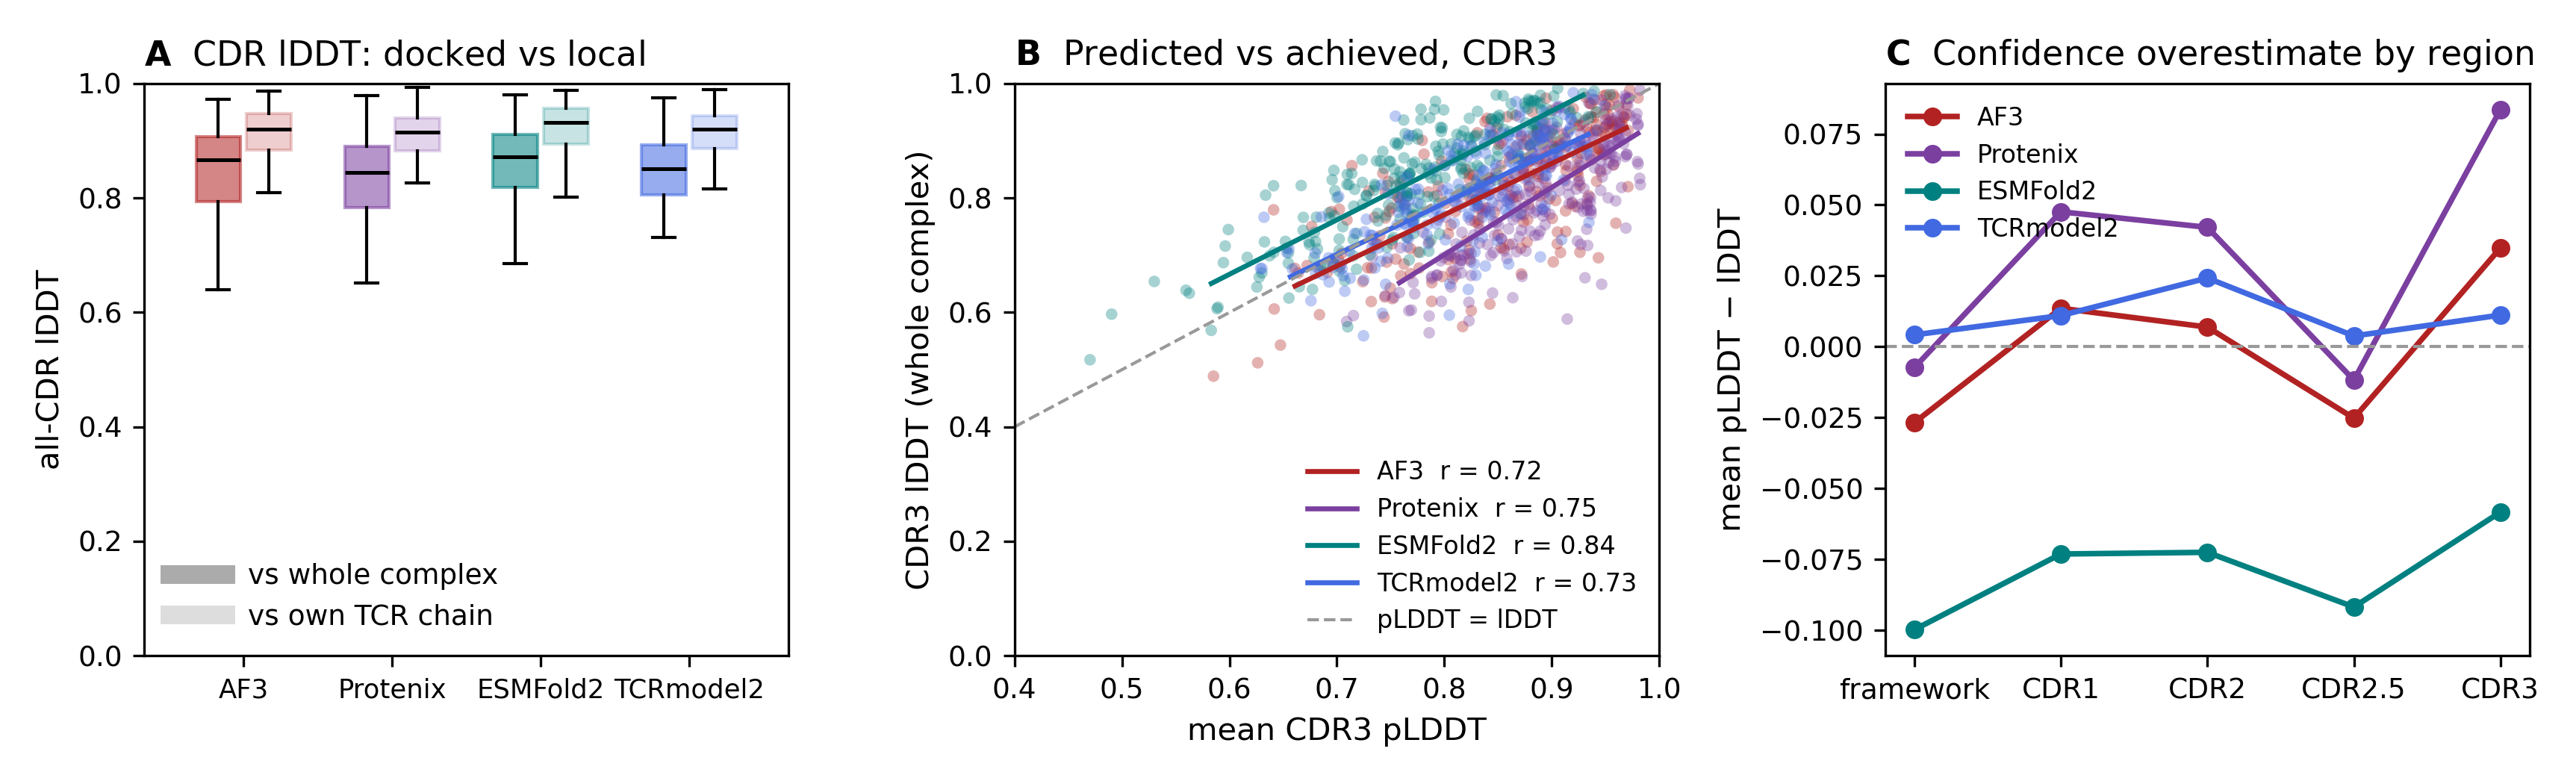
\includegraphics[width=1\linewidth,height=\textheight,keepaspectratio,alt={Superposition-free CDR accuracy and the models' own confidence. (A) All-CDR C-alpha lDDT with the whole complex as contact partners and with the CDR's own TCR chain only. (B) Mean CDR3 pLDDT against the CDR3 lDDT achieved, CDR3-alpha and CDR3-beta pooled, with per-method linear fits and Pearson r; the dashed line is perfect calibration. (C) Mean pLDDT minus lDDT by region, framework through CDR3.}]{Figure_lddt.png}
\caption{\textbf{Superposition-free CDR accuracy and the models' own
confidence.} (\textbf{A}) All-CDR C\ensuremath{\alpha} lDDT with the whole
complex as contact partners (dark) and with the CDR's own TCR chain only
(pale). Removing the docking raises every method by a similar amount and
compresses the differences between them. (\textbf{B}) Mean CDR3 pLDDT
against the CDR3 lDDT actually achieved, CDR3\ensuremath{\alpha} and
CDR3\ensuremath{\beta} pooled, with per-method linear fits and Pearson
\emph{r}; the dashed line is perfect calibration. (\textbf{C}) Mean
pLDDT − lDDT by region. Three of the four methods cross from understating
the framework to overstating CDR3; ESMFold2 is conservative
everywhere.}
\end{figure}

\subsection{3.6 Effect of MHC class}\label{effect-of-mhc-class}

Class II is not harder than class I on this benchmark (Figure 4C).
Median Global DockQ for class II versus class I is 0.752 versus 0.750
(AlphaFold 3), 0.742 versus 0.736 (ESMFold2) and 0.713 versus 0.698
(Protenix); every difference is well inside the spread, and the class II
subset is small (n = 15). ESMFold2's class II mean (0.743) is its
highest subgroup mean. We note this mainly as a caution: with 15 class
II complexes, this benchmark cannot resolve a class effect of the size
other studies report, and the TCRmodel2 comparison is class I only by
construction.

\subsection{3.7 Effect of reference
resolution}\label{effect-of-reference-resolution}

Accuracy declines with worsening reference resolution for every method,
but not equally (Figure 4B). Pearson r between resolution and Global
DockQ is \ensuremath{-}0.292 for AlphaFold 3 (p = 0.001), \ensuremath{-}0.266 for ESMFold2 (p =
0.003), \ensuremath{-}0.238 for TCRmodel2 (p = 0.012) and \ensuremath{-}0.184 for Protenix (p =
0.040, Spearman p = 0.065, not significant). Part of this is unavoidable
--- a lower-resolution reference is a noisier target --- but the
ordering is informative: the two methods most sensitive to reference
quality are the two most accurate ones, which is what one expects if the
residual error in the best models is approaching the coordinate
uncertainty of the references themselves.

\subsection{3.8 Confidence calibration and reference-free quality
scores}\label{confidence-calibration-and-reference-free-quality-scores}

Interface confidence predicts accuracy for all three general methods,
but ESMFold2's ipTM does so substantially better (Figure 4A). Pearson r
between ipTM and Global DockQ is 0.793 for ESMFold2 (Spearman \ensuremath{\rho} =
0.777), against 0.660 for AlphaFold 3 (\ensuremath{\rho} = 0.654) and 0.657 for Protenix
(\ensuremath{\rho} = 0.679). The regression lines also differ in intercept: ESMFold2
reaches a given DockQ at a systematically lower ipTM than the other two,
so its confidence is both more conservative and better ordered. pDockQ
shows the same ranking with lower correlations overall (ESMFold2 r =
0.676, Protenix 0.611, AlphaFold 3 0.577).

\begin{figure}
\centering
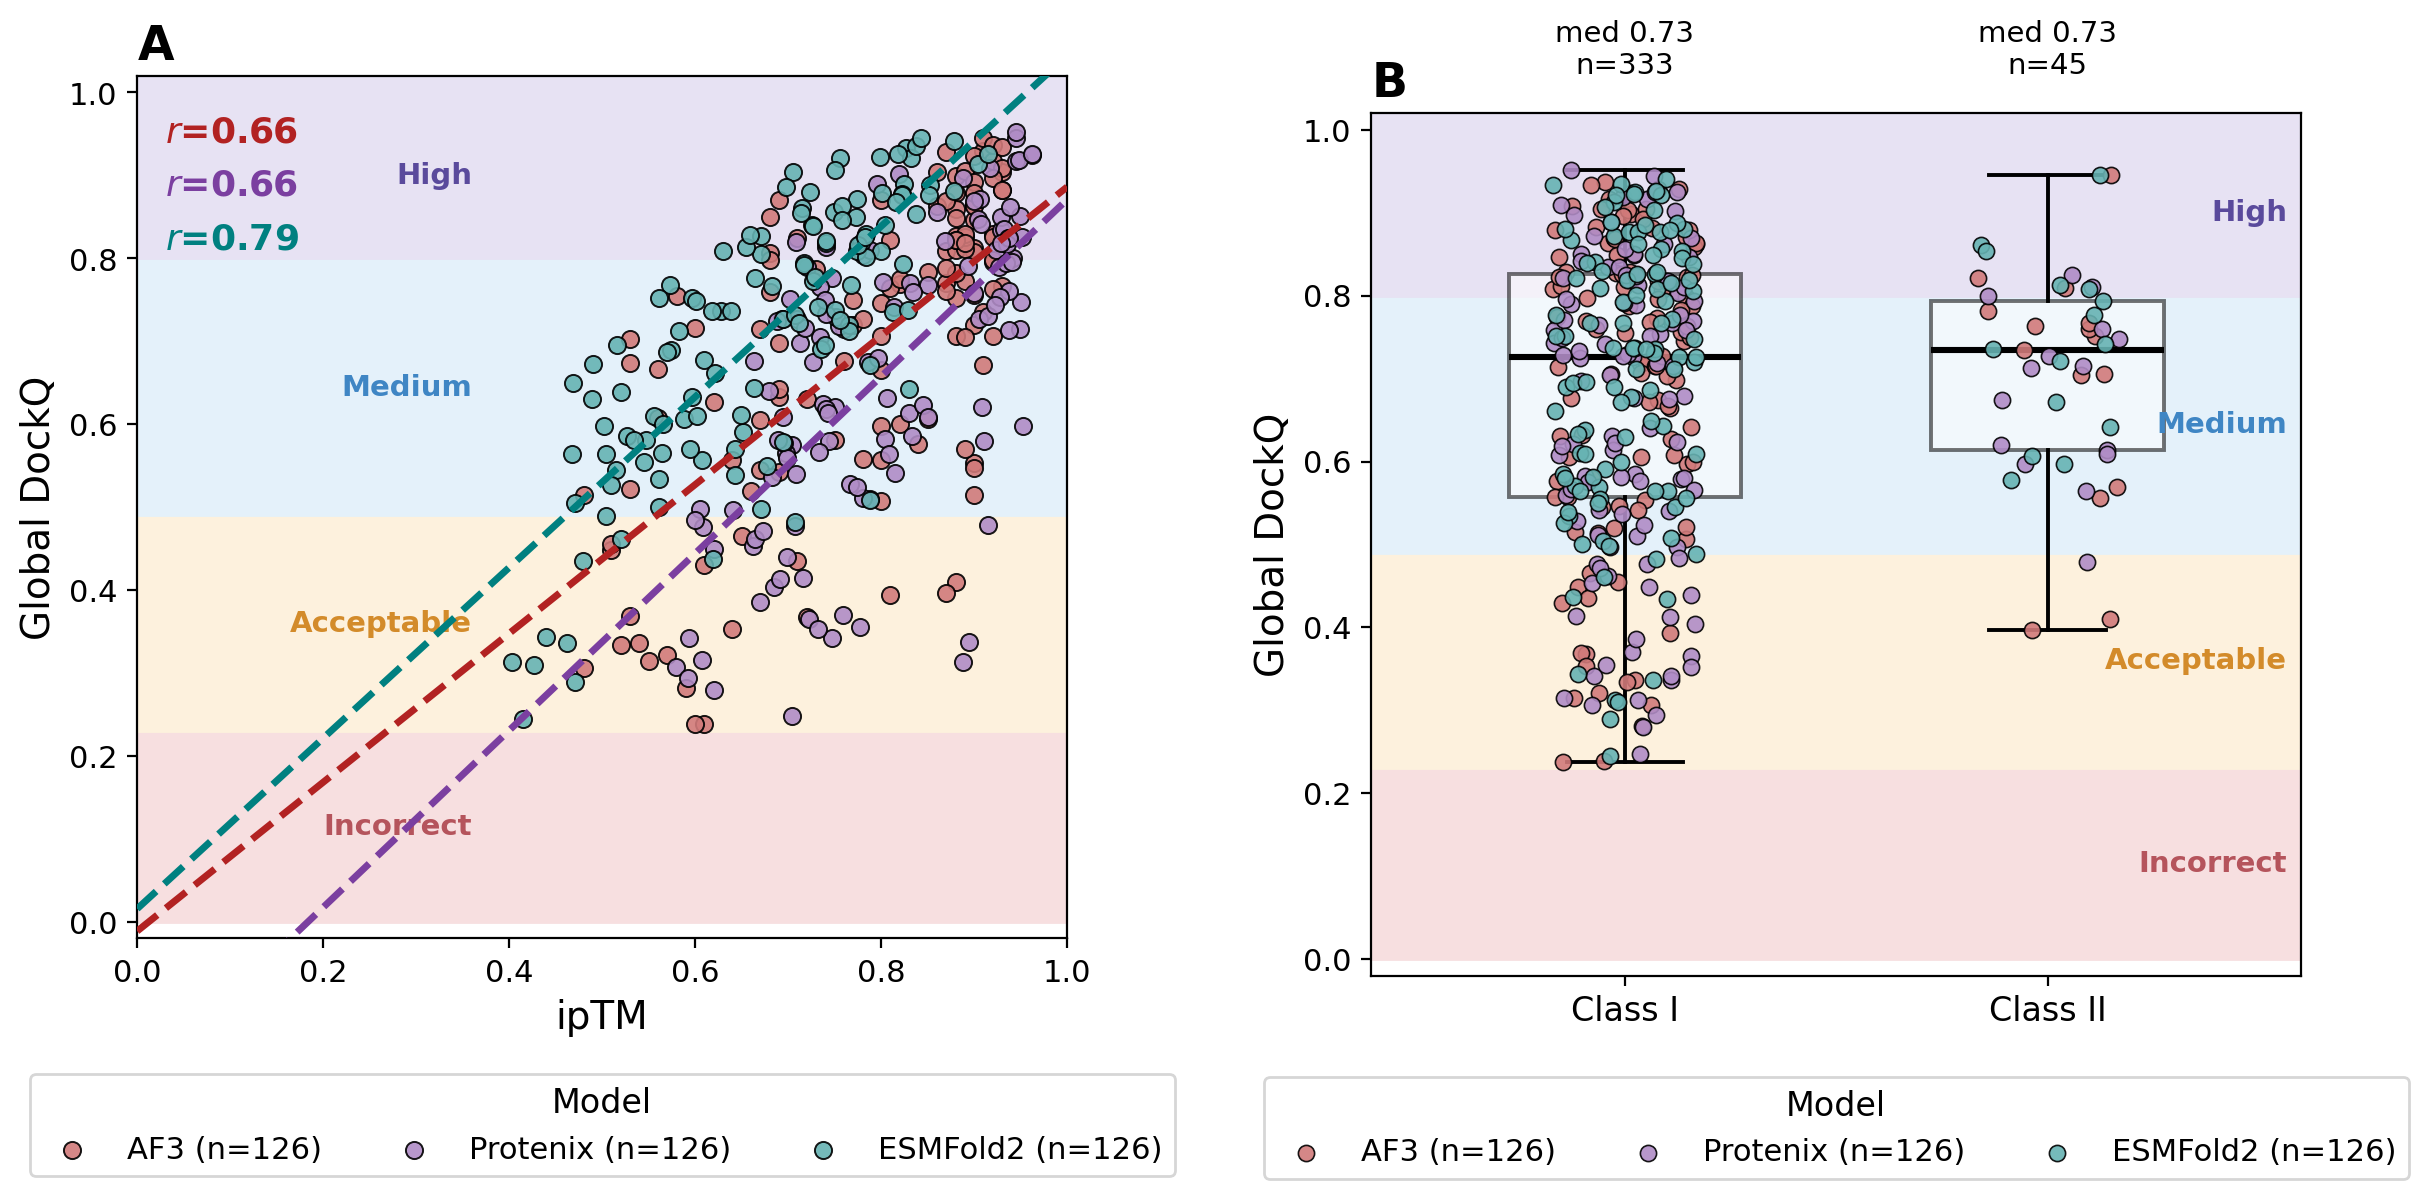
\includegraphics[width=1\linewidth,height=\textheight,keepaspectratio,alt={Determinants of interface accuracy. (A) Global DockQ against each method's own ipTM, with per-method linear fits and Pearson r. ESMFold2's confidence is both more conservative --- it reaches a given DockQ at a lower ipTM --- and better ordered. (B) Global DockQ against the resolution of the experimental reference. (C) Global DockQ by MHC class. Shaded bands are the CAPRI quality classes.}]{Figure_determinants.png}
\caption{\textbf{Determinants of interface accuracy.} (\textbf{A})
Global DockQ against each method's own ipTM, with per-method linear fits
and Pearson \emph{r}. ESMFold2's confidence is both more conservative
--- it reaches a given DockQ at a lower ipTM --- and better ordered.
(\textbf{B}) Global DockQ against the resolution of the experimental
reference. (\textbf{C}) Global DockQ by MHC class. Shaded bands are the
CAPRI quality classes.}
\end{figure}

\subsection{3.9 A composite single-prediction score beats the published
classifier}\label{a-composite-single-prediction-score-beats-the-published-classifier}

For AlphaFold 3 specifically, single global confidence scores leave
accuracy on the table. Replacing ipTM with the weakest \emph{pairwise}
ipTM already raises Pearson r from 0.660 to 0.695 over all 126
complexes, and the four-term composite of Section 2.10 --- computed from
one AlphaFold 3 prediction, with no second structure and no reference
--- reaches r = 0.712 (95\% CI 0.617--0.791) and \ensuremath{\rho} = 0.725
(0.624--0.803) (Figure 5A).

It is the best of the scores available for an AlphaFold 3 prediction
(Figure 5B). On the same 126 complexes the published random-forest quality-tier
classifier [11] reaches r = 0.662 (\ensuremath{\rho} = 0.674), AlphaFold 3's own ipTM
0.660 (0.654) and pDockQ 0.660 (0.679) --- that is, the classifier does
no better than the two confidence scores it was built to improve on. The
paired difference between the composite and the classifier is +0.050
Pearson (95\% bootstrap CI +0.015 to +0.085) and +0.051 Spearman (+0.008
to +0.098), so the advantage over all 126 complexes excludes zero on
both metrics.

That margin narrows on every subset. On the 111 class I
complexes the composite reaches r = 0.738 and \ensuremath{\rho} = 0.760 against the
classifier's 0.700 and 0.734, a paired +0.038 Pearson (CI +0.004 to
+0.072) but +0.027 Spearman (\ensuremath{-}0.013 to +0.067). On the 27 class I
targets whose PDB identifiers are absent from the classifier's training
set the two are indistinguishable, and the sign is not even consistent:
+0.021 Pearson (\ensuremath{-}0.080 to +0.129) and \ensuremath{-}0.047 Spearman (\ensuremath{-}0.187 to
+0.078). The 15 class II complexes favour the composite by +0.082 on
both metrics, with intervals several times wider than the effect.

Two things follow. The composite is the better ranking of AlphaFold 3
predictions across this benchmark, but its formula was fixed on this
benchmark, and 27 unseen targets cannot separate it from the classifier;
we therefore do not claim a resolved advantage for any single-model
score on unseen targets. And all of these scores --- learned or not ---
are beaten by a quantity that needs no quality model at all
(Section 3.11).

\begin{figure}
\centering
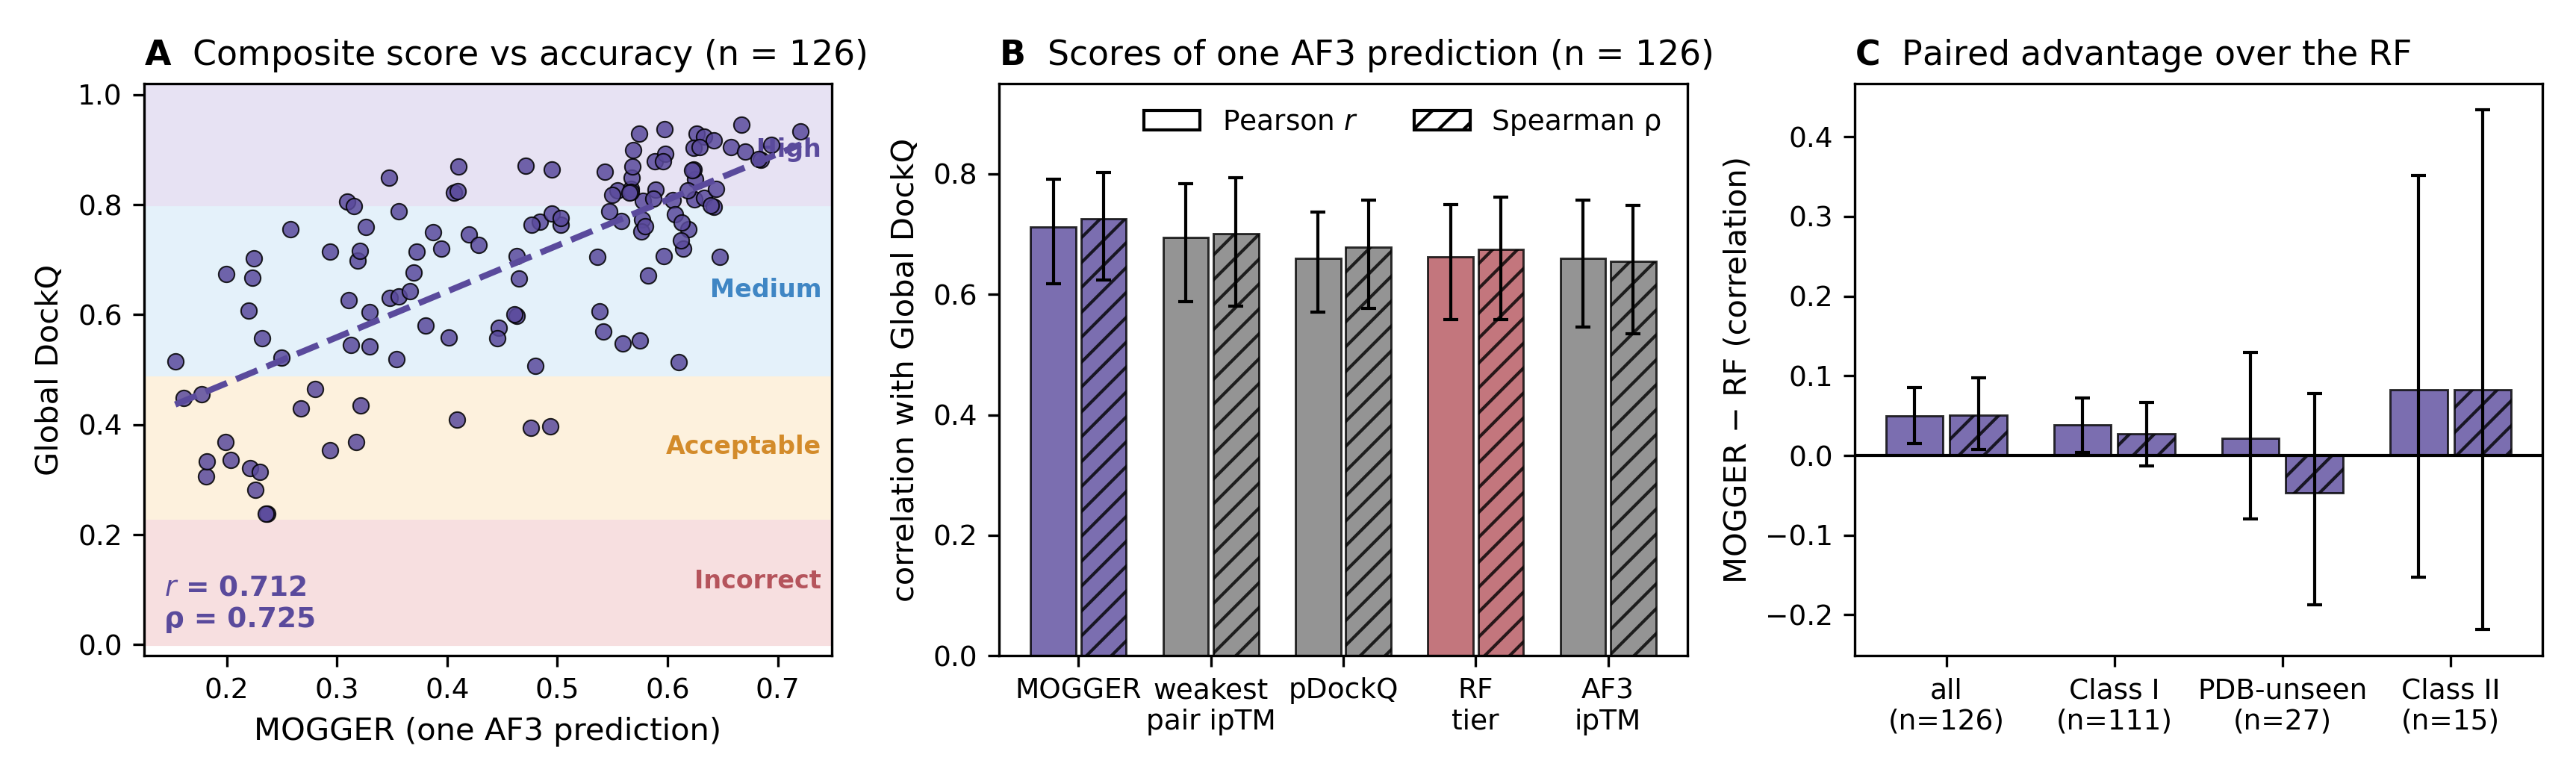
\includegraphics[width=1\linewidth,height=\textheight,keepaspectratio,alt={The composite single-prediction confidence score against the published alternatives. (A) Global DockQ against the composite score for the 126 complexes, with the linear fit and both correlations; shaded bands are the CAPRI quality classes. (B) Pearson r and Spearman rho with Global DockQ for every score computable from one AlphaFold 3 prediction, over all 126 complexes; whiskers are 95 percent bootstrap intervals. }]{Figure_mogger.png}
\caption{\textbf{A composite single-prediction score against the
published alternatives.} (\textbf{A}) Global DockQ against MOGGER for
the 126 complexes, with the linear fit and both correlations; shaded
bands are the CAPRI quality classes. (\textbf{B}) Correlation with
Global DockQ for every score computable from one AlphaFold 3
prediction, over all 126 complexes;
whiskers are 95\% bootstrap intervals.}
\end{figure}

\subsection{3.10 Effect of similarity to pre-cutoff
structures}\label{effect-of-similarity-to-pre-cutoff-structures}

Accuracy rises weakly but significantly with similarity to the
pre-cutoff structural record. Pooled over 245 predictions, the strongest
single predictor is not any individual chain but the composite mean
identity over the closest \emph{complete} pre-cutoff complex (Spearman \ensuremath{\rho}
= +0.271, p = 1.8 \ensuremath{\times} 10\ensuremath{^{-}}\ensuremath{^{5}}); the individual components are weaker (TCR\ensuremath{\beta}
+0.192, peptide +0.151, TCR\ensuremath{\alpha} +0.127, MHC +0.059, n.s.). The full
pre-specified model (DockQ \textasciitilde{} method + TCR\ensuremath{\alpha} + TCR\ensuremath{\beta} +
peptide + MHC + class) explains 7.2\% of the variance (adjusted R\ensuremath{^{2}} =
0.048), with TCR\ensuremath{\beta} identity worth +0.041 DockQ per 10 identity points (p
= 0.024) and peptide identity +0.015 (p = 0.005). Between the extreme
bins of the composite score, mean DockQ rises from 0.515 to 0.702
(AlphaFold 3) and 0.438 to 0.661 (Protenix).

The negative MHC coefficient in that model is an artefact of no variance
rather than evidence that MHC familiarity hurts: MHC identity has median
100\% and IQR 99.4--100\%, because 111 of 126 targets are class I HLA
alleles whose peptide-binding domain is in the PDB many times over. A
useful counterexample: two targets have a 100\%-identical complete
pre-cutoff complex --- 7RTR (identical to 7N1F) and 9NDS (identical to
4FTV) --- and AlphaFold 3 still scores 7RTR at only 0.36, CAPRI
acceptable. Sequence-level availability of the answer does not guarantee
a good prediction.

The threshold sweep matters for how method comparisons should be read.
Filtering at \ensuremath{\leq} 95\% maximum TCR identity retains 69 targets and barely
moves absolute accuracy (AlphaFold 3 mean DockQ 0.585 \ensuremath{\rightarrow} 0.547; Protenix
0.515 \ensuremath{\rightarrow} 0.506), but it dissolves the AlphaFold 3--over--Protenix result:
the paired advantage falls from +0.063 (p = 0.031) to +0.027 (p = 0.40),
and at \ensuremath{\leq} 90\% it reverses sign. Below 95\% the retained samples (14, 7
and 1 targets) are too small to conclude anything either way. We
therefore conclude that the AlphaFold 3 advantage over Protenix on this
benchmark is carried by targets with a near-duplicate TCR in the
pre-cutoff PDB. It is also the reason we did not build the primary
benchmark on a TCR-identity filter: only 7 of 126 targets fall below
70\% identity, and those 7 are not ``hard targets'' but mostly unusual
or non-human TCRs.

\subsection{3.11 Structural divergence between AlphaFold 3 and
ESMFold2}\label{structural-divergence-between-alphafold-3-and-esmfold2}

Equal accuracy is not the same as equal predictions. Across the 126
complexes the median C\ensuremath{\alpha} RMSD between the AlphaFold 3 and ESMFold2
predictions of the same FASTA is 1.35 \AA{}, but the distribution runs to
13.9 \AA{}, and the disagreement is anatomically specific. The two models
agree closely on everything except where the TCR sits: median peptide
RMSD in the MHC frame is 0.44 \AA{} and median peptide conformation RMSD is
0.33 \AA{}, and the median internal RMSD of the TCR module itself is 0.74 \AA{}
--- but the median MHC--TCR\ensuremath{\alpha} and MHC--TCR\ensuremath{\beta} interface RMSDs are 1.62 and
1.63 \AA{}, and the rigid-body decomposition gives a median TCR rotation of
11.1\ensuremath{^{\circ}} with a tail reaching 177\ensuremath{^{\circ}}. On 20 of 126 complexes the two models
place the TCR more than 30\ensuremath{^{\circ}} apart, and on 10 of them more than 90\ensuremath{^{\circ}}
apart, while building the same pMHC and the same TCR fold. The
disagreement is a docking disagreement, not a folding one.

The disagreement is also bimodal rather than graded. Of the 126
complexes, 106 place the TCR within 30\ensuremath{^{\circ}} of each other and only 12 exceed
60\ensuremath{^{\circ}}; there is essentially nothing in between, and those 12 are exactly the
12 largest cross-model RMSDs. Superposing each prediction's MHC on the
native's and measuring its TCR against the native's separates the two
models on these cases: among the 20 complexes that disagree by more than
30\ensuremath{^{\circ}}, AlphaFold 3 is the misplaced one on 12, ESMFold2 on 4, and both are
misdocked on 4. Over the 10 largest disagreements the median Global
DockQ is 0.335 for AlphaFold 3 and 0.581 for ESMFold2, and only 2 of the
10 have both models at medium-or-better accuracy, against 101 of the
remaining 116. Where the two architectures disagree about docking, at
least one of them has failed, and it is usually AlphaFold 3.

Two geometrically distinct failures produce the disagreement. In the
first, the misplaced TCR is rotated 100--177\ensuremath{^{\circ}} \emph{and} translated
50--63 \AA{}: it is not docked on the groove at all but on another surface of
the MHC, still burying 55--150 C\ensuremath{\alpha} contacts there while making no contact
with the peptide (9EJG, 8RYO, 7RK7, 7PB2; the fifth such case, 9EJH, is
the inverse --- its native TCR is the one docked away from the peptide,
and AlphaFold 3 builds the canonical peptide-centred pose instead). In the second,
the TCR still straddles the groove and still contacts the peptide, but
is turned around on it: 70--177\ensuremath{^{\circ}} of rotation with the centre of mass only
4--12 \AA{} from where the other model puts it, a reversal of docking
polarity rather than a relocation (9RU5, 8ES9, 7RM4, 7RRG, 9NW2).

The relocations have a specific and avoidable cause. Projecting the TCR
centre on the axis from the MHC centre to the peptide centre places the
native TCR 28.8 \AA{} above the peptide-binding platform in the median
complex, and no class I native below 14 \AA{}. Three predictions --- 8RYO, 7RK7 and 7PB2,
all AlphaFold 3, all class I --- put the TCR 24--26 \AA{} \emph{below} the
platform, docked on the \ensuremath{\beta}-sheet floor that in the intact molecule is
covered by the \ensuremath{\alpha}3 domain and \ensuremath{\beta}2-microglobulin and that the domain
truncation of Section 2.2 leaves exposed. On these three complexes
AlphaFold 3 scores 0.28, 0.24 and 0.31 while ESMFold2, given the same
truncated input, scores 0.91, 0.53 and 0.63 and places the TCR within
3--19\ensuremath{^{\circ}} of the native. Part of AlphaFold 3's tail of docking failures is
therefore an artefact of presenting it with a non-physiological surface,
not a failure to recognise the correct one --- a caveat that applies to
any truncated-input benchmark, and one ESMFold2 appears not to share.

That disagreement is a strong, entirely reference-free predictor of
accuracy (Figure 6A). Cross-model C\ensuremath{\alpha} RMSD correlates with AlphaFold 3's
Global DockQ at Spearman \ensuremath{\rho} = \ensuremath{-}0.756 and with ESMFold2's at \ensuremath{\rho} = \ensuremath{-}0.670,
and with the \emph{worse} of the two at \ensuremath{\rho} = \ensuremath{-}0.884 (p = 1.1 \ensuremath{\times} 10\ensuremath{^{-}}\ensuremath{^{4}}\ensuremath{^{2}}).
For comparison, on the same 126 complexes AlphaFold 3's own ipTM
predicts that worse-of-two value at \ensuremath{\rho} = +0.604 and ESMFold2's at \ensuremath{\rho} =
+0.639. Cross-architecture agreement is therefore a better native-free
quality signal than either model's internal confidence, than pDockQ, and
than the composite and random-forest scores of Section 3.9 --- and it
requires no confidence head, no training, and no calibration.

By divergence quartile (Figure 6B), median Global DockQ falls from 0.860
(AlphaFold 3) and 0.862 (ESMFold2) in the most-agreeing quartile to
0.518 and 0.564 in the most-divergent one. Notably, the two models
mostly fail on the \emph{same} complexes: both quartile trends are
parallel, and among the 20 most divergent complexes, 4 are failed by
both at the medium threshold while 12 are solved by exactly one.

The residual complementarity is nonetheless substantial (Figure 6C). At
DockQ \ensuremath{\geq} 0.49, AlphaFold 3 succeeds on 107 of 126 complexes and ESMFold2
on 115; the two together succeed on 119 (103 both, 4 AlphaFold 3 only,
12 ESMFold2 only, 7 neither). Pooling an MSA-based and a
language-model-based predictor therefore raises the medium-or-better
rate from 85\% or 91\% to 94\% --- echoing the pooling gains Yin et
al.~report for antibody--peptide complexes [13] --- and, because
disagreement itself flags the failures, the pool comes with a built-in
triage signal.

Two related class II entries illustrate the pattern concretely. 7SG1 and
7SG2 are HLA-DQ2 complexes with closely related gluten-derived peptides.
On 7SG2 both models are correct (AlphaFold 3 0.706, ESMFold2 0.642) and
their predictions differ by 2.72 \AA{} with a 14\ensuremath{^{\circ}} TCR rotation. On 7SG1 the
models diverge by 3.56 \AA{} with a 26\ensuremath{^{\circ}} rotation, and AlphaFold 3 drops to
0.396 while ESMFold2 holds at 0.736. Both models report high confidence
on both complexes (AlphaFold 3 ipTM 0.87 and 0.92; ESMFold2 0.81 and
0.83) --- the confidence heads do not see the failure, and the
disagreement does.

\begin{figure}
\centering

\includegraphics[width=1\linewidth,height=\textheight,keepaspectratio,alt={Structural divergence between the AlphaFold 3 and ESMFold2 predictions. (A) C\ensuremath{\alpha} RMSD between the AlphaFold 3 and ESMFold2 predictions of the same sequence against the worse of their two Global DockQ scores. (B) Global DockQ by quartile of that divergence; the two methods degrade together. (C) Complexes reaching medium-or-better accuracy: individually, jointly, and neither.}]{Figure_divergence.png}
\caption{\textbf{Structural divergence between the AlphaFold 3 and
ESMFold2 predictions.} (\textbf{A}) C\ensuremath{\alpha} RMSD between the AlphaFold 3 and
ESMFold2 predictions of the same sequence against the worse of their two
Global DockQ scores. (\textbf{B}) Global DockQ by quartile of that
divergence; the two methods degrade together. (\textbf{C}) Complexes
reaching medium-or-better accuracy: individually, jointly, and neither.}
\end{figure}

\subsection{3.12 Denoising trajectories of the two
samplers}\label{denoising-trajectories-of-the-two-samplers}

Instrumenting both diffusion samplers on the same complexes shows that
the equality of outcome conceals very different dynamics (Figure 7A).
AlphaFold 3 begins denoising from an initial noise scale of
\textasciitilde2,560 \AA{} and is still \textasciitilde44 \AA{} from the native
at the midpoint of its 200-step schedule; ESMFold2 begins at
\textasciitilde256 \AA{} and is already within \textasciitilde5.7 \AA{} at its
own midpoint. Measured as the fraction of the schedule at which the
trajectory comes permanently within 1 \AA{} of its own final frame,
AlphaFold 3 converges at 73\% of its steps and ESMFold2 at 58\%.
AlphaFold 3 spends most of its schedule in a regime where, at the scale
the noise schedule sets, no structure has settled at all; ESMFold2
commits early and refines.

The same behaviour at scale (Figure 7B, 30 complexes \ensuremath{\times} 5 samples =
30,000 recorded frames) puts AlphaFold 3's convergence in a narrow
window. Mean C\ensuremath{\alpha} RMSD to the final frame of the same sample falls below
2.0 \AA{} at step 150 and below 1.0 \AA{} at step 158; every complex is within
1.0 \AA{} by step 159; accuracy against the native plateaus at 3.37 \AA{} around
step 163; and mean RMSD to the final frame falls below 0.5 \AA{} at step
164. Four independent criteria land between steps 150 and 164 of 200.
For roughly the first 140 steps the state is noise at the scale the
schedule sets --- AlphaFold 3's schedule holds \ensuremath{\sigma} above 5 \AA{} until
\textasciitilde70\% of the way through.

\subsection{3.13 Effect of AlphaFold 3 sampler settings on accuracy and
runtime}\label{effect-of-alphafold-3-sampler-settings-on-accuracy-and-runtime}

If the trajectory has effectively converged by step \textasciitilde160,
the last 40 steps and the four extra diffusion samples should be nearly
free to remove. They are (Figure 7C, Table 4). Over the same 30
complexes, same MSAs, same seeds, run serially on one idle GPU:

\begin{longtable}[]{@{}
  >{\raggedright\arraybackslash}p{(\linewidth - 12\tabcolsep) * \real{0.1092}}
  >{\raggedright\arraybackslash}p{(\linewidth - 12\tabcolsep) * \real{0.1429}}
  >{\raggedright\arraybackslash}p{(\linewidth - 12\tabcolsep) * \real{0.1849}}
  >{\raggedleft\arraybackslash}p{(\linewidth - 12\tabcolsep) * \real{0.0924}}
  >{\raggedleft\arraybackslash}p{(\linewidth - 12\tabcolsep) * \real{0.1597}}
  >{\raggedright\arraybackslash}p{(\linewidth - 12\tabcolsep) * \real{0.2101}}
  >{\raggedleft\arraybackslash}p{(\linewidth - 12\tabcolsep) * \real{0.1008}}@{}}
\caption{\textbf{AlphaFold 3 sampler economy on 30 complexes.} Same
complexes, same MSAs and templates, same per-complex seed, run serially
on one idle RTX PRO 6000. Confidence intervals are paired bootstrap;
\emph{p} values are paired tests against the baseline track. GPU seconds
are mean \ensuremath{\pm} SD over the 30 complexes and exclude a constant 3.3 s of CPU
featurisation.}\tabularnewline
\toprule\noalign{}
\begin{minipage}[b]{\linewidth}\raggedright
Track
\end{minipage} & \begin{minipage}[b]{\linewidth}\raggedright
Steps \ensuremath{\times} samples
\end{minipage} & \begin{minipage}[b]{\linewidth}\raggedright
GPU s per prediction
\end{minipage} & \begin{minipage}[b]{\linewidth}\raggedleft
Speed-up
\end{minipage} & \begin{minipage}[b]{\linewidth}\raggedleft
Mean Global DockQ
\end{minipage} & \begin{minipage}[b]{\linewidth}\raggedright
\ensuremath{\Delta} vs baseline (95\% CI)
\end{minipage} & \begin{minipage}[b]{\linewidth}\raggedleft
Paired \emph{p}
\end{minipage} \\
\midrule\noalign{}
\endfirsthead
\toprule\noalign{}
\begin{minipage}[b]{\linewidth}\raggedright
Track
\end{minipage} & \begin{minipage}[b]{\linewidth}\raggedright
Steps \ensuremath{\times} samples
\end{minipage} & \begin{minipage}[b]{\linewidth}\raggedright
GPU s per prediction
\end{minipage} & \begin{minipage}[b]{\linewidth}\raggedleft
Speed-up
\end{minipage} & \begin{minipage}[b]{\linewidth}\raggedleft
Mean Global DockQ
\end{minipage} & \begin{minipage}[b]{\linewidth}\raggedright
\ensuremath{\Delta} vs baseline (95\% CI)
\end{minipage} & \begin{minipage}[b]{\linewidth}\raggedleft
Paired \emph{p}
\end{minipage} \\
\midrule\noalign{}
\endhead
\bottomrule\noalign{}
\endlastfoot
Baseline & 200 \ensuremath{\times} 5 & 10.04 \ensuremath{\pm} 0.03 & 1.00\ensuremath{\times} & 0.7212 & --- & --- \\
Fewer steps & 160 \ensuremath{\times} 5 & 8.79 \ensuremath{\pm} 0.03 & 1.14\ensuremath{\times} & 0.7143 & \ensuremath{-}0.007 (\ensuremath{-}0.026,
+0.007) & 0.43 \\
One sample & 200 \ensuremath{\times} 1 & 6.02 \ensuremath{\pm} 0.01 & 1.67\ensuremath{\times} & 0.7143 & \ensuremath{-}0.007 (\ensuremath{-}0.021,
+0.006) & 0.34 \\
Both & 160 \ensuremath{\times} 1 & 5.57 \ensuremath{\pm} 0.01 & \textbf{1.80\ensuremath{\times}} & 0.7109 & \ensuremath{-}0.010 (\ensuremath{-}0.032,
+0.007) & 0.33 \\
\end{longtable}

Every confidence interval straddles zero, no track loses a complex from
the acceptable band (30/30 everywhere), and the high-accuracy fraction
moves from 0.367 to 0.333 --- one complex. Adding the constant 3.3 s of
CPU featurisation gives the end-to-end figure: 13.4 s \ensuremath{\rightarrow} 8.9 s per
complex, or 401 s \ensuremath{\rightarrow} 267 s for all 30. Note that the 160-step track is
not the 200-step trajectory stopped early --- AlphaFold 3 re-discretises
the same \ensuremath{\sigma} range into 160 coarser steps --- so this is an experiment
testing the convergence analysis, not a restatement of it.

The speed-up saturates at 1.8\ensuremath{\times} for a structural reason. Fitting \emph{t}
= trunk + \emph{c} \ensuremath{\times} (steps \ensuremath{\times} samples) across all 120 timed predictions
gives a fixed trunk of 4.86 s and 5.08 ms per sample-step (R\ensuremath{^{2}} = 0.995).
Half of a default AlphaFold 3 run on a complex of this size is the
Pairformer trunk and its 10 recycles, which neither shortcut touches;
driving diffusion cost to zero would give at most 1.9\ensuremath{\times}. Dropping from
five samples to one also costs the ranking step --- AlphaFold 3 normally
returns the best of five by ranking score --- and on this sample that
selection is worth \ensuremath{-}0.007 DockQ, which is not detectable at n = 30.

\begin{figure}
\centering
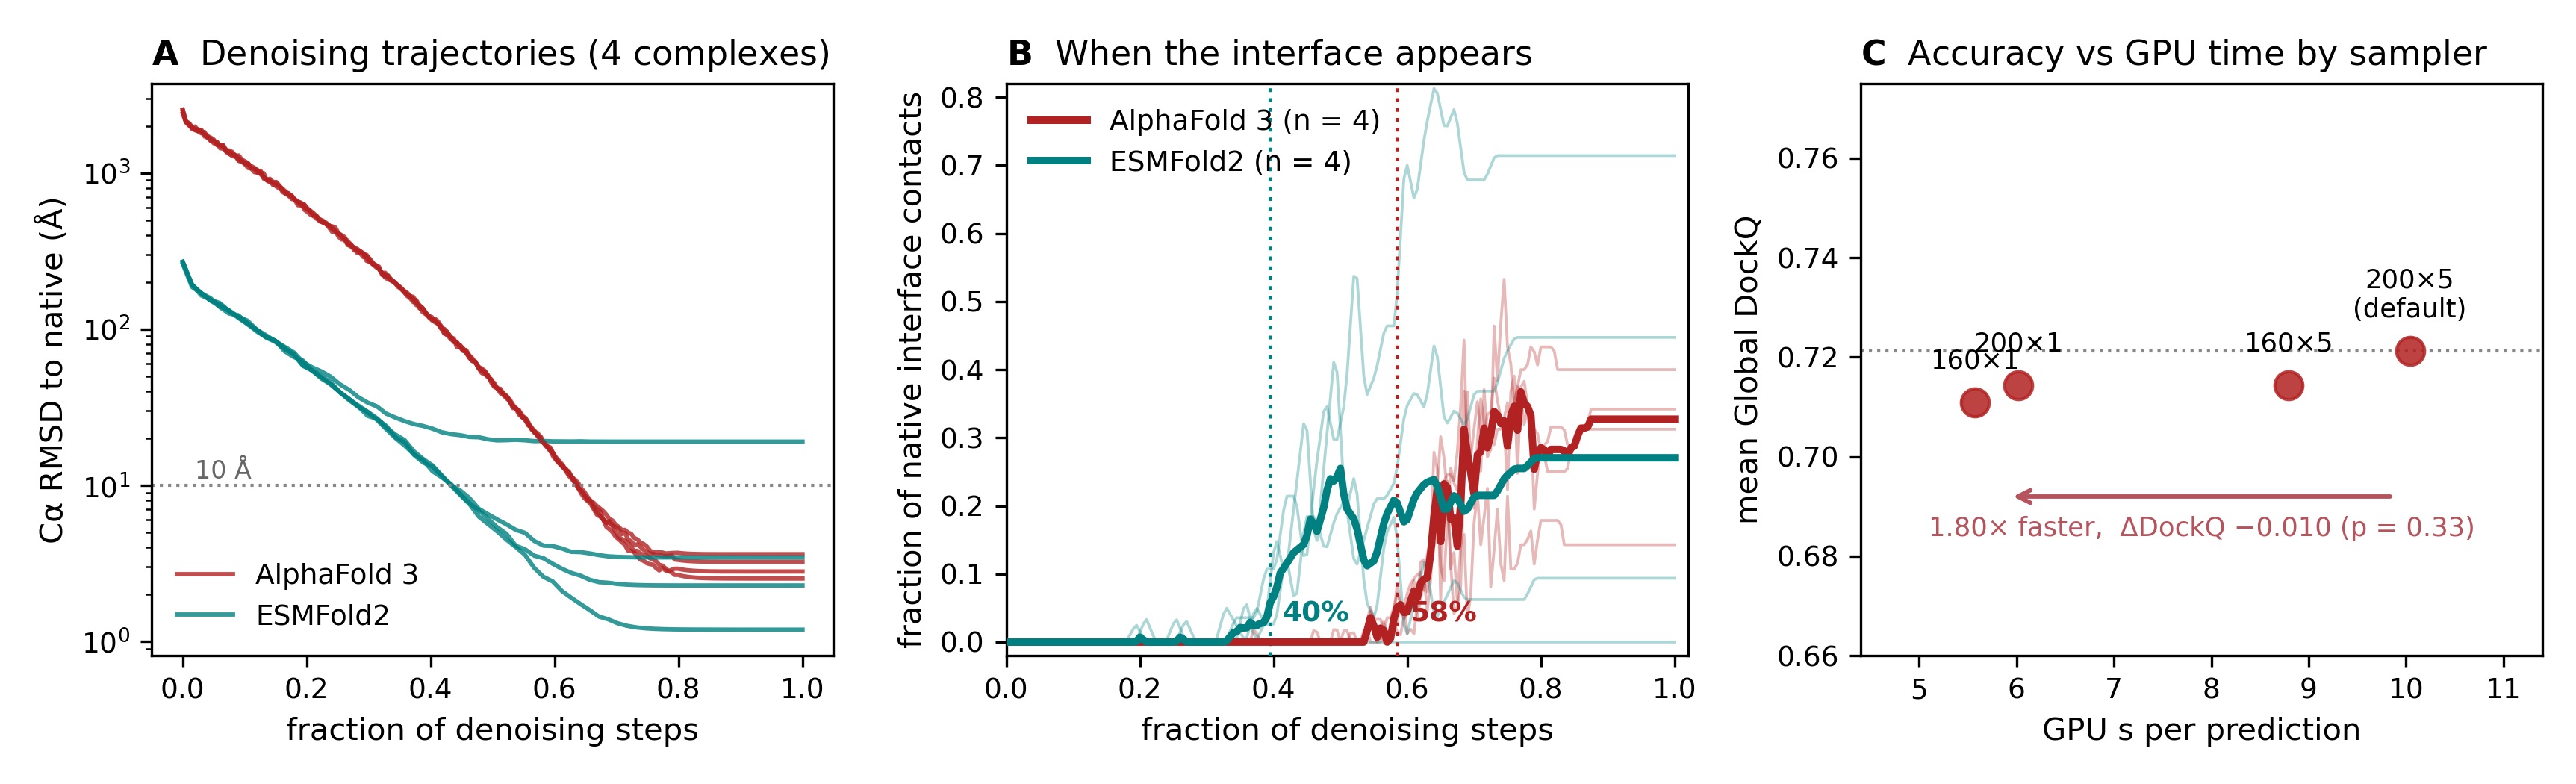
\includegraphics[width=1\linewidth,height=\textheight,keepaspectratio,alt={Denoising trajectories and AlphaFold 3 sampler economy. (A) C\ensuremath{\alpha} RMSD to the native along the denoising trajectory for four complexes traced in both models; AlphaFold 3 (200 steps, initial \ensuremath{\sigma} \ensuremath{\approx} 2,560 \AA{}) is still tens of \aa{}ngströms out at its midpoint, ESMFold2 (68 recorded steps, initial \ensuremath{\sigma} \ensuremath{\approx} 256 \AA{}) is within a few \aa{}ngströms. (B) AlphaFold 3 convergence to its own final frame over 30 complexes \ensuremath{\times} 5 samples; band spans median to 90th percentile. (C) GPU time against mean Global DockQ for four sampler configurations on the same 30 complexes.}]{Figure_sampler.png}
\caption{\textbf{Denoising trajectories and AlphaFold 3 sampler
economy.} (\textbf{A}) C\ensuremath{\alpha} RMSD to the native along the denoising
trajectory for four complexes traced in both models; AlphaFold 3 (200
steps, initial \ensuremath{\sigma} \ensuremath{\approx} 2,560 \AA{}) is still tens of \aa{}ngströms out at its
midpoint, ESMFold2 (68 recorded steps, initial \ensuremath{\sigma} \ensuremath{\approx} 256 \AA{}) is within a
few \aa{}ngströms. (\textbf{B}) AlphaFold 3 convergence to its own final
frame over 30 complexes \ensuremath{\times} 5 samples; band spans median to 90th
percentile. (\textbf{C}) GPU time against mean Global DockQ for four
sampler configurations on the same 30 complexes.}
\end{figure}

\section{4 Discussion}\label{discussion}

\subsection{4.1 Multiple sequence alignments are not required for
TCR--pMHC
modelling}\label{multiple-sequence-alignments-are-not-required-for-tcrpmhc-modelling}

The clearest result reported here is a negative one: on 126 post-cutoff
complexes, a diffusion predictor conditioned only on a protein language
model matched AlphaFold 3 running with server-supplied MSAs and
templates (median Global DockQ 0.736 vs 0.751, paired p = 0.68), and
exceeded it in the fraction of medium-or-better models (91.3\% vs
84.9\%). This differs from the current consensus [10,11]. The
discrepancy appears to be generational rather than contradictory: the
PLM predictors in those comparisons are ESMFold-generation models whose
structure module descends from AlphaFold 2, whereas ESMFold2 pairs a
6-billion-parameter language model with a diffusion structure head. The
most informative data point in Lu et al.~is that their best-performing
PLM method was the one built on an AlphaFold-3-style architecture
[10]; the present result is the same observation with the
architecture gap closed further. Why this should hold for this problem
in particular is worth stating explicitly: TCR variable domains and MHC
platforms are among the most heavily sequenced and most heavily
crystallised folds in existence, so an MSA adds little that a large
language model has not already internalised, whereas the quantity an MSA
cannot supply --- the relative orientation of two domains with no
coevolutionary history with one another --- is precisely what remains
unsolved.

\subsection{4.2 Docking, not loop conformation, is the unsolved
problem}\label{docking-not-loop-conformation-is-the-unsolved-problem}

The per-interface decomposition and the two CDR metrics point the same
way. MHC--peptide interfaces are modelled at DockQ \ensuremath{\approx} 0.94 by all four
methods; CDR3 loops are built to within 1.6--2.3 \AA{} heavy-atom RMSD of
the native by all four after framework alignment, with a spread across
methods of half an \aa{}ngström. Docking accuracy, by contrast, spans tens
of \aa{}ngströms, is right-skewed with catastrophic outliers, and accounts
for essentially all of the difference between methods and between
complexes. This reproduces the decomposition Shi et al.~reported
[12] on a larger and more recent set, and it argues that further
progress on TCR--pMHC modelling will come from the placement problem,
not from loop refinement.

\subsection{4.3 Cross-architecture agreement as a reference-free quality
signal}\label{cross-architecture-agreement-as-a-reference-free-quality-signal}

The C\ensuremath{\alpha} RMSD between an AlphaFold 3 and an ESMFold2 prediction of the
same sequence predicted the worse of their two DockQ scores at \ensuremath{\rho} =
\ensuremath{-}0.884, against +0.60 to +0.64 for the models' own ipTM values,
\textasciitilde0.68 for pDockQ, and \textasciitilde0.67--0.73 for
learned quality scores. This is not a subtle effect and it is cheap: one
extra prediction from a method that runs in five seconds. It also has a
mechanistic reading. Two models that share a generative head but nothing
on the conditioning side have largely independent failure modes for the
docking problem, so their agreement is evidence in a way that a single
model's self-reported confidence --- which, as 7SG1 shows, can be high
on a wrong answer --- is not. A practical consequence follows: for
TCR--pMHC modelling campaigns, running both architectures, using their
agreement as a triage score, and taking the union of their predictions
raises the medium-or-better rate on this benchmark from 85\% (AlphaFold
3 alone) to 94\%.

\subsection{4.4 Sampler settings and computational
cost}\label{sampler-settings-and-computational-cost}

AlphaFold 3's denoising trajectory has converged to within 1 \AA{} of its
own answer by step 158 of 200, and running with 160 steps and a single
diffusion sample returned the answer in 55\% of the GPU time with no
detectable accuracy cost over 30 complexes. The scope of that result
should be emphasised: n = 30, one GPU, one seed per complex, and one
narrow size regime (397--416 residues, all in AlphaFold 3's 512-token
bucket). Larger complexes shift the trunk/diffusion split --- the trunk
scales roughly quadratically in the pair track while diffusion scales
with atom count --- so the 1.9\ensuremath{\times} ceiling moves. Within this regime,
though, the finding is straightforward: for high-throughput TCR--pMHC
screening the default settings buy almost nothing, and the compute is
better spent on a second architecture, which Section 3.11 shows is worth
considerably more than a fifth diffusion sample.

\subsection{4.5 Implications for benchmark
design}\label{implications-for-benchmark-design}

Two methodological points generalise beyond this set. First, native
construction is not a solved preprocessing step. Forty-six of 136
entries are built from files holding several complete complexes, and the
deposited asymmetric unit is often not a complex; six natives required a
biological-assembly fetch or a periodic-boundary repair, and one (9J4S)
had no physical TCR--pMHC interface in any author-defined assembly, its
apparent interface being a lattice contact between two copies. A
contact-count check cannot catch this --- only requiring all chains to
come from a single author-defined assembly does. A benchmark that scores
such an entry is scoring noise. Second, redundancy filtering on TCR
identity is less informative than it appears for this class of complex:
germline V-gene framework dominates a \textasciitilde110-residue
variable domain, so 119 of 126 targets sit above 70\% identity to
something pre-cutoff, and the \ensuremath{\leq} 90\% subset is 14 mostly non-human or
atypical TCRs rather than a representative hard set. The composite
identity to the closest \emph{complete} pre-cutoff complex separates the
benchmark far better and at usable sample sizes (46 targets have no
complete pre-cutoff match at all). We report both, and we report
explicitly that the AlphaFold 3--over--Protenix result does not survive
a 95\% TCR-identity filter, which is the kind of statement benchmark
papers should make routinely.

\subsection{4.6 Limitations}\label{limitations}

The class II subset (n = 15) is too small to resolve class effects, and
TCRmodel2 was run on class I only because it accepts a fixed class II
peptide length. Nine entries were excluded for non-standard peptide
chemistry or covalent tethering, both of which are biologically
interesting categories that sequence-input prediction currently cannot
address, so their exclusion reflects a limitation of the methods as much
as of the benchmark. ``Training set'' is a proxy throughout --- neither
AlphaFold 3's nor Protenix's actual training list is public, and we use
PDB availability on or before 30 September 2021 as the closest
reproducible stand-in, which cannot account for sequence databases or
non-TCR structures the models also saw. The reference set for that
analysis is only as complete as TCR3d \ensuremath{\cup} STCRDab. AlphaFold 3 and
Protenix were run through public servers, so their exact data pipelines
are outside our control; ESMFold2 was likewise run through the ESM SDK
API, and the trajectory analysis of Section 3.12 used the local
\texttt{biohub/ESMFold2} checkpoint rather than the API model, so its
per-frame DockQ values are not interchangeable with the benchmark's. The
composite confidence score of Section 3.9 was developed on this
benchmark and requires independent validation. Finally, the
sampler-economy result is a single-seed, single-GPU, 30-complex
experiment in one size regime, as stated above.

\section{5 Conclusions}\label{conclusions}

On 126 TCR--pMHC complexes released after the shared 30 September 2021
training cutoff, a single-sequence protein-language-model diffusion
predictor matched AlphaFold 3 and beat an AlphaFold 3 reproduction, with
no MSA and no structural template. Both, and a TCR-specialised AlphaFold
2 derivative, build the pMHC and the CDR3 loops to comparable accuracy
and differ almost entirely in where they place the TCR. The disagreement
between the two architectures is anatomically confined to that
placement, and predicts accuracy better than any of the confidence
scores evaluated here, so that a two-architecture ensemble is both more
accurate (94\% versus 85\% medium-or-better) and self-triaging.
AlphaFold 3's denoising trajectory converges by step 158 of 200, and
reducing the sampler to 160 steps and one diffusion sample returns the
same answers in 55\% of the GPU time. Taken together, these observations
favour running two architectures at reduced sampler settings over a
single architecture at default settings, and using the agreement between
them to identify which predictions can be relied upon.

\section{Data and code availability}\label{data-and-code-availability}

The benchmark inputs (136 truncated FASTAs, chain manifests, review
records), the rebuilt experimental references and their provenance
manifest, all predictions, and the complete scoring, analysis and figure
code are contained in the accompanying repository. Per-interface DockQ
results are provided in long format (one row per interface plus Global
DockQ), TCR CDR RMSD results per prediction with full coverage and
quality-control columns, CDR lDDT and pLDDT in long format (one row per
prediction and region, both contact sets), the sampler-economy tracks with per-complex
timings and paired differences, and the per-structure confidence features
and bootstrap intervals behind the composite score of Section 2.10. All analyses are reproducible from the
recorded commands; software versions and model checkpoint revisions and
hashes are recorded in the accompanying manifests.

\section{References}\label{references}

\begin{enumerate}
\def\labelenumi{\arabic{enumi}.}
\tightlist
\item
  Gowthaman R, Pierce BG. TCR3d: The T cell receptor structural
  repertoire database. \emph{Bioinformatics} 2019;35(24):5323--5325.
  doi:10.1093/bioinformatics/btz517
\item
  Leem J, de Oliveira SHP, Krawczyk K, Deane CM. STCRDab: the structural
  T-cell receptor database. \emph{Nucleic Acids Res}
  2018;46(D1):D406--D412. doi:10.1093/nar/gkx971
\item
  Lin V, Cheung M, Gowthaman R, Eisenberg M, Baker BM, Pierce BG. TCR3d
  2.0: expanding the T cell receptor structure database with new
  structures, tools and interactions. \emph{Nucleic Acids Res}
  2025;53(D1):D604--D608. doi:10.1093/nar/gkae840
\item
  Jumper J, Evans R, Pritzel A, et al.~Highly accurate protein structure
  prediction with AlphaFold. \emph{Nature} 2021;596(7873):583--589.
  doi:10.1038/s41586-021-03819-2
\item
  Yin R, Feng BY, Varshney A, Pierce BG. Benchmarking AlphaFold for
  protein complex modeling reveals accuracy determinants. \emph{Protein
  Sci} 2022;31(8):e4379. doi:10.1002/pro.4379
\item
  Abramson J, Adler J, Dunger J, et al.~Accurate structure prediction of
  biomolecular interactions with AlphaFold 3. \emph{Nature}
  2024;630(8016):493--500. doi:10.1038/s41586-024-07487-w
\item
  Bradley P. Structure-based prediction of T cell receptor:peptide-MHC
  interactions. \emph{eLife} 2023;12:e82813. doi:10.7554/eLife.82813
\item
  Yin R, Ribeiro-Filho HV, Lin V, Gowthaman R, Cheung M, Pierce BG.
  TCRmodel2: high-resolution modeling of T cell receptor recognition
  using deep learning. \emph{Nucleic Acids Res} 2023;51(W1):W569--W576.
  doi:10.1093/nar/gkad356
\item
  Lin Z, Akin H, Rao R, et al.~Evolutionary-scale prediction of
  atomic-level protein structure with a language model. \emph{Science}
  2023;379(6637):1123--1130. doi:10.1126/science.ade2574
\item
  Lu J, Zhu X, Hu X, Zhang C, Feng F. Benchmarking TCR--pMHC structure
  prediction: a unified evaluation and CDR3-based functional insights.
  \emph{Brief Bioinform} 2026;27(3):bbag289. doi:10.1093/bib/bbag289
\item
  Ascunce-París A, Romero-Durana M, Valencia A, Farriol-Duran R, Guallar
  V. Structural quality-tier assessment for TCR-pMHC functional
  enrichment. \emph{Front Immunol} 2026;17:1869810.
  doi:10.3389/fimmu.2026.1869810
\item
  Shi Y, Parks JM, Smith JC. Comparative analysis of TCR and TCR-pMHC
  complex structure prediction tools. \emph{J Chem Inf Model}
  2025;65(13):7156--7173. doi:10.1021/acs.jcim.5c00298
\item
  Yin R, Saravanakumar S, Shi SY, et al.~Benchmarking AlphaFold and
  related deep learning approaches for modeling antibody and TCR antigen
  recognition. \emph{bioRxiv} 2026:2026.07.04.736425.
  doi:10.64898/2026.07.04.736425
\item
  Basu S, Wallner B. DockQ: a quality measure for protein-protein
  docking models. \emph{PLoS One} 2016;11(8):e0161879.
  doi:10.1371/journal.pone.0161879
\item
  Mirabello C, Wallner B. DockQ v2: improved automatic quality measure
  for protein multimers, nucleic acids, and small molecules.
  \emph{Bioinformatics} 2024;40(10):btae586.
  doi:10.1093/bioinformatics/btae586
\item
  Lensink MF, Brysbaert G, Raouraoua N, et al.~Impact of AlphaFold on
  structure prediction of protein complexes: the CASP15-CAPRI
  experiment. \emph{Proteins} 2023;91(12):1658--1683.
  doi:10.1002/prot.26609
\item
  Dunbar J, Deane CM. ANARCI: antigen receptor numbering and receptor
  classification. \emph{Bioinformatics} 2016;32(2):298--300.
  doi:10.1093/bioinformatics/btv552
\item
  Lefranc MP, Pommié C, Ruiz M, et al.~IMGT unique numbering for
  immunoglobulin and T cell receptor variable domains and Ig superfamily
  V-like domains. \emph{Dev Comp Immunol} 2003;27(1):55--77.
  doi:10.1016/s0145-305x(02)00039-3
\item
  Woods LJ, Neff B, Lahouel K, et al.~General prediction of T cell
  receptor antigen specificity from sequence using AlphaFold 3.
  \emph{bioRxiv} 2026:2026.06.02.729478. doi:10.64898/2026.06.02.729478
\item
  Bryant P, Pozzati G, Elofsson A. Improved prediction of
  protein-protein interactions using AlphaFold2. \emph{Nat Commun}
  2022;13(1):1265. doi:10.1038/s41467-022-28865-w
\item
  ESMFold2 model release, \texttt{biohub/ESMFold2} (revision
  \texttt{8fc3ff47}) with \texttt{biohub/ESMC-6B} (revision
  \texttt{45b0fa5d}), accessed via the ESM SDK, model
  \texttt{esmfold2-fast-2026-05}.
\item
  Protenix: an open reproduction of the AlphaFold 3 architecture
  (ByteDance AML AI4Science), run through the public Protenix server.
\item
  Mariani V, Biasini M, Barbato A, Schwede T. lDDT: a local
  superposition-free score for comparing protein structures and models
  using distance difference tests. \emph{Bioinformatics}
  2013;29(21):2722--2728. doi:10.1093/bioinformatics/btt473
\end{enumerate}

\end{document}
